\documentclass[11pt]{article}

% Editorial objective for AI collaborators and future revisions:
% develop this manuscript as an initial six-page IEEE Control Systems Letters
% (L-CSS) publication, followed by an expanded L-CSS + ACC version for
% presentation at ACC. The alternative conference path is L-CSS + CDC 2027;
% in either case, L-CSS is intended to be the archival journal publication.

\usepackage[margin=1in]{geometry}

\usepackage{amsmath,amssymb,amsthm}
\usepackage{graphicx}
\usepackage{booktabs}
\usepackage{float}
\usepackage[hidelinks]{hyperref}
\usepackage{cite}
\newtheorem{lemma}{Lemma}
\newtheorem{theorem}{Theorem}
\newtheorem{proposition}{Proposition}
\newtheorem{corollary}{Corollary}
\newtheorem{remark}{Remark}

\begin{document}

\title{A Theory of Information Architecture for Networked Decisions:
Freshness, Locality, and Coordination}
\author{Scott Moeller and Bhaskar Krishnamachari}

\date{August 2026}

\hypersetup{
  pdftitle={A Theory of Information Architecture for Networked Decisions: Freshness, Locality, and Coordination},
  pdfauthor={Scott Moeller and Bhaskar Krishnamachari},
  pdfsubject={Decision-relevant information scope and freshness in networked static teams},
  pdfkeywords={information architecture, networked decisions, static teams, age of information, distributed coordination}
}

\maketitle

\begin{abstract}
Networked decisions often face a structural tradeoff: broader information
improves coordination but generally arrives with greater delay. We formalize an
\emph{information architecture} as specifying what each agent knows, from
where, and at what age, and measure its performance by \emph{architecture
regret}, the loss relative to the full-information decision. First, we compare
fresh-local with stale-global information. The crossover is governed by
decision-relevant temporal predictability and the share of decision-relevant
variation captured by local information. Under a common-rate Gauss--Markov model with affine
full-information decisions, this yields a closed-form threshold in the
dimensionless delay $\tau/T$. Second, for a synchronized-snapshot radius family
in which broader neighborhood snapshots arrive at greater age, we characterize
the optimal radius within that family by balancing marginal spatial-information
gain against marginal freshness loss. In a canonical field
model, the resulting scaling depends on the spatial correlation length
$\ell_s$, decision-relevance length $\ell_c$, and temporal propagation length
$L_T=vT$. Numerical experiments recover the predicted local--global crossover,
zero-to-positive-radius threshold, interior optimal-radius behavior, and
corresponding shifts on finite noncanonical graphs. Within the analyzed
exogenous-state quadratic framework, architecture performance is governed by
predictability of the full-information decision rather than state-prediction
accuracy alone.
\end{abstract}

\section{Introduction}
\label{sec:introduction}

Many networked systems must repeatedly make coupled decisions using information
that is distributed across space and changes over time. A wireless transmitter
may know its current local channel state but not the current interference
conditions elsewhere in the network; an edge server may observe its own
workload immediately while a system-wide view is available only after telemetry
has been collected and disseminated; and a distributed sensing system may have
fresh measurements from nearby sensors while observations from distant sensors
arrive with greater latency. In each case, broad information can improve
coordination, but obtaining it takes time. The resulting design choice is not
simply between centralized and distributed control, but between
\emph{information architectures} that differ simultaneously in spatial scope
and temporal freshness.

This tension is familiar in several literatures, but its different aspects have
largely been studied separately. Work on stale information in distributed
systems has shown that old global state can lose much of its value and can even
lead to poor load-balancing decisions \cite{mitzenmacher2000old}. The Age of
Information literature formalizes freshness as a system resource and studies
how communication and queueing determine the timeliness of available state
\cite{kaul2012realtime}. Distributed optimization, in contrast, canonically
studies how agents compute a global solution under a specified communication
graph and information-exchange mechanism \cite{nedic2009distributed}.
Organizational economics has identified a closely related
adaptation--coordination tradeoff: decentralized decision makers adapt directly
to local conditions, whereas centralized decisions facilitate coordination at
the cost of communicating dispersed information
\cite{alonso2008coordination}. These perspectives all suggest that neither
``local'' nor ``global'' information is intrinsically preferable. What matters
is whether the additional coordination enabled by broader information is worth
the loss in freshness required to obtain it.

This paper develops a theory for this tradeoff. We consider a collection of
agents operating in an exogenously evolving stochastic environment
$\theta_t=(\theta_{1,t},\ldots,\theta_{n,t})$. At each decision epoch the agents
select a joint action $x_t=(x_{1,t},\ldots,x_{n,t})$ that incurs a common cost
$f(x_t,\theta_t)$. An \emph{information architecture} specifies the information
available to each agent when this decision is made. Thus a fresh-local
architecture may allow agent $i$ to condition on the current $\theta_{i,t}$,
a neighborhood architecture may provide the states of agents within a given
spatial radius, and a global architecture may provide the entire state vector
only after a delay $\tau$. More generally, an architecture specifies
\emph{who knows what, from where, and at what age}.

Our analysis uses the classical fixed-information framework of static team
decision theory initiated by Radner \cite{radner1962team}. In the
deterministic-Hessian quadratic model considered here, completing the square
reduces optimization under any fixed information architecture to a
Hilbert-space approximation problem: the team-optimal policy is the
$Q$-orthogonal projection of the full-information action onto the closed
subspace of implementable policies. Consequently, the architecture regret is
\begin{equation}
    R(\mathcal A)
    =
    \frac{1}{2}
    \left\|
        x_t^\star-\Pi_{\mathcal S(\mathcal A)}x_t^\star
    \right\|_Q^2 ,
    \label{eq:intro_projection}
\end{equation}
where $\mathcal S(\mathcal A)$ denotes the admissible policy subspace. We use
this fixed-architecture specialization as an analytical primitive and study an
outer structured comparison/design problem in which spatial scope and
information age vary jointly. Classical team and information-structure work
has also treated information and organizational networks as design objects
\cite{marschak1972economic,summers2017information}. The narrower question
pursued here is how scope-dependent age changes the value of a
synchronized-snapshot radius family when information is evaluated through
prediction error of the full-information decision.

Classical team theory established fixed-information optimality conditions and
also treated the value and organization of information, while later work has
designed measurement or communication structures and studied radius-limited
local information \cite{marschak1972economic,summers2017information,
rusmevichientong2003decentralized}. Networked-control work has likewise
examined controller scope coupled to architecture-dependent latency
\cite{ballotta2023latency}. Our contribution is narrower: in an
exogenous-state quadratic static-team model, we couple the scope of a
synchronized snapshot to its age and value the resulting information through
prediction error of the full-information decision. This yields the
pure-benchmark crossover, the common-rate spatio-temporal composition identity,
and the coordination-radius characterization for the structured
scope--latency family.

Our first result answers the two extreme points of this tradeoff. We compare a
\emph{fresh-local} architecture, in which each agent observes its current local
state, against a \emph{stale-global} architecture, in which every agent has
access to the complete system state with delay $\tau$. In general, the loss
from staleness is governed by the prediction error of the current
decision-relevant state from information $\tau$ units old. For a
Gauss--Markov environment with temporal coherence time $T$, and for an affine
full-information decision, the global architecture has the exact regret
\begin{equation}
    R_{\mathrm{glob}}(\tau)
    =
    \left(1-e^{-2\tau/T}\right)R_\infty ,
    \label{eq:intro_global}
\end{equation}
where $R_\infty$ is the regret of the best open-loop decision. If
$R_{\mathrm{loc}}$ denotes fresh-local regret and
\begin{equation}
    \eta_{\mathrm{loc}}
    \triangleq
    1-\frac{R_{\mathrm{loc}}}{R_\infty}
\end{equation}
is the fraction of decision-relevant variation explainable from fresh-local
information, then fresh-local decisions outperform stale-global decisions
exactly when
\begin{equation}
    \frac{\tau}{T}
    >
    \frac{1}{2}\log\frac{1}{\eta_{\mathrm{loc}}}.
    \label{eq:intro_crossover}
\end{equation}
Thus the value of global coordination is controlled by two independent
quantities: how rapidly global information loses predictive value in time, and
how much of the globally optimal decision is already predictable locally. For
a canonical shared-resource quadratic model with local stiffness $q$ and
coordination strength $\gamma$, the large-system threshold reduces to
\begin{equation}
    \left(\frac{\tau}{T}\right)^\star
    =
    \frac{1}{2}\log\left(1+\frac{\gamma}{q}\right),
    \label{eq:intro_coupling}
\end{equation}
making explicit how stronger decision coupling increases the amount of
staleness that is worth tolerating in exchange for global coordination.

The local--global comparison concerns two pure benchmark regimes. Our second
result considers agents embedded in a graph or spatial domain and a
synchronized-snapshot family in which each agent bases its decision on a
time-aligned neighborhood snapshot of radius $r$. Increasing $r$ replaces a
narrower, fresher snapshot by a broader snapshot of greater age $\tau(r)$.
The resulting architecture faces two
competing sources of error: a \emph{spatial omission error}, caused by
excluding decision-relevant state beyond radius $r$, and a
\emph{temporal staleness error}, caused by the delay required to acquire the
broader information.

We characterize this tradeoff using the spatial and temporal predictability of
the underlying stochastic field. In a canonical model, spatial dependence is
described by a correlation length $\ell_s$, temporal variation by a coherence
time $T$, and communication by the scope--delay relation $\tau(r)$. We show
that the optimal radius within the synchronized-snapshot family
\begin{equation}
    r^\star
    \in
    \arg\min_r R\!\left(\mathcal A_{r,\tau(r)}\right)
    \label{eq:intro_rstar}
\end{equation}
is determined jointly by these environmental scales and by the coupling
structure of the decision objective. The result yields comparative statics
with direct architectural interpretations: faster temporal variation favors
smaller and fresher information radii; faster information propagation supports
broader coordination; and stronger long-range decision coupling increases the
value of larger information scope. Spatial smoothness determines how rapidly
additional spatial observations become redundant and hence how much
information radius is needed to approximate global decisions. Under tractable
spatio-temporal covariance and propagation models, these effects combine into
dimensionless scaling laws for $r^\star$.

The distinction between \emph{state predictability} and
\emph{decision-relevant predictability} is important. A remote state variable
may be difficult to predict yet irrelevant to the optimal action, while a small
uncertainty in another variable may matter greatly because of strong coupling
in the objective. Our results therefore weight spatio-temporal uncertainty by
its effect on the full-information decision. This makes the appropriate
coordination scale a property not only of the stochastic environment, but of
the combination of the environment, the decision problem, and the
communication architecture.

The framework deliberately separates information architecture from the
algorithm used to implement it. It consequently complements canonical
distributed-optimization formulations, where the communication structure is
specified first and the principal question is how to compute efficiently over it
\cite{nedic2009distributed}. We study a structured outer comparison over a
scope--age family. Similarly, unlike freshness metrics that
assign value to an update primarily through its age
\cite{kaul2012realtime}, the value of an observation here depends on how much
it changes the downstream decision. This perspective also suggests extensions
to heterogeneous information radii, sparse long-range information
``shortcuts,'' low-dimensional global summaries, and budget-constrained
information acquisition.

Our model is intentionally restricted to \emph{static} information structures:
the stochastic environment may be temporally and spatially correlated, but
agents' current actions do not alter the information subsequently observed by
other agents. This boundary is consequential. Once actions influence future
observations, they may serve simultaneously as control actions and implicit
signals, leading to the nonclassical dynamic-team phenomena highlighted by
Witsenhausen's counterexample \cite{witsenhausen1968counterexample}. Thus the
present theory is most directly applicable to repeated networked optimization
against an exogenously evolving environment---for example, stylized quadratic
or locally quadratic models of rate, power, compute, or sensing decisions
driven by changing demand, channel, or resource conditions---rather than to
fully constrained engineering formulations, controlled queueing, or
decentralized Markov decision processes.

In summary, this paper makes two technical contributions and one conceptual
contribution:
\begin{enumerate}
    \item We derive an exact \emph{fresh-local versus stale-global crossover
    law} that quantifies when the adaptation advantage of fresh-local
    information exceeds the coordination advantage of delayed global
    information.

    \item We develop a \emph{coordination-scale law} for the
    synchronized-snapshot radius family under the stated common-rate model,
    characterizing its optimal spatial scope as a function of temporal
    predictability, spatial predictability, communication latency, and decision
    coupling.

    \item We show that, within the analyzed framework, architecture performance is governed by
    \emph{decision-relevant predictability}, not raw state predictability. The
    desired architecture depends jointly on environmental statistics, decision
    sensitivity and coupling, information geometry, and freshness; the
    communication graph and decision geometry therefore need not coincide.
\end{enumerate}

Together, these results support normalized comparisons within a structured
family that goes beyond a binary choice between centralized and distributed
decision making. Within that family, the preferred radius is the spatial scale
at which the marginal value of broader coordination is balanced by the loss of
information freshness required to obtain it.

%```latex
\section{Networked Decisions and Information Architectures}
\label{sec:model}

We consider a network of decision-making agents operating in a stochastic
environment whose state is distributed across the network and evolves over
time. Our formulation separates three distinct objects: the
\emph{network geometry}, which defines relationships and distances among
agents; the \emph{decision problem}, which determines how their actions and
states interact in the objective; and the \emph{information architecture},
which determines what information is available to each agent and with what
delay. These three structures need not coincide.

The environment evolves exogenously: agents react to the state but their
current actions do not alter the law governing its future evolution. The model
therefore describes repeated information-constrained decisions rather than a
controlled Markov process. Under the fixed-information static-team
formulation, the present deterministic-Hessian quadratic model admits the
projection characterization developed below. We use that fixed-architecture
result as the inner optimization primitive for comparing structured
scope--age architectures.

\subsection{Network, Environment, and Decision Model}
\label{subsec:decision_model}

There are $n$ decision-making agents indexed by
\[
    V=\{1,\ldots,n\},
\]
represented as the vertices of a graph
\begin{equation}
    G=(V,E).
    \label{eq:network_graph}
\end{equation}
The graph provides a notion of network or spatial proximity. We write
$d_G(i,j)$ for the graph distance between nodes $i$ and $j$, and define the
radius-$r$ neighborhood of node $i$ as
\begin{equation}
    \mathcal{N}_r(i)
    \triangleq
    \{j\in V:d_G(i,j)\le r\}.
    \label{eq:r_neighborhood}
\end{equation}
Depending on the application, $G$ may represent a physical communication
network, a geographic neighborhood relation, or another structure governing
the cost or latency of obtaining nonlocal information.
\footnote{The graph model is adopted for concreteness. The framework can more
generally be formulated for agents embedded in a metric space, or for any
collection of agents equipped with a meaningful notion of neighborhoods and
information-propagation cost.}

Let
\[
    \theta=\{\theta_t\}_{t\in\mathbb{T}}
\]
be a stochastic process defined on a probability space
$(\Omega,\mathcal{F},\mathbb{P})$, where $\mathbb{T}$ may be discrete or
continuous. At time $t$, the environment state is
\begin{equation}
    \theta_t
    =
    \left(
        \theta_{1,t},\ldots,\theta_{n,t}
    \right)
    \in\mathbb{R}^{m},
    \qquad
    \theta_{i,t}\in\mathbb{R}^{m_i},
    \qquad
    \sum_{i=1}^{n}m_i=m .
    \label{eq:state_partition}
\end{equation}
The component $\theta_{i,t}$ denotes the state locally associated with node
$i$. Depending on the application, it may represent a local channel
condition, workload or demand, sensing quality, resource availability, or
another externally evolving quantity relevant to the decision.

For the basic results in this section, we assume that $\theta_t$ is stationary
and square-integrable:
\begin{equation}
    \mathbb{E}\|\theta_t\|^2<\infty.
    \label{eq:state_integrability}
\end{equation}
No independence, Gaussianity, Markov property, or specific form of spatial or
temporal correlation is required. More structured stochastic models will be
introduced later when we derive explicit architecture laws.

Agent $i$ chooses an action
\[
    x_{i,t}\in\mathbb{R}^{d_i},
\]
and the joint action is
\begin{equation}
    x_t
    =
    (x_{1,t},\ldots,x_{n,t})
    \in\mathbb{R}^{d},
    \qquad
    d=\sum_{i=1}^{n}d_i .
    \label{eq:joint_action}
\end{equation}

The agents share a common per-stage cost
\begin{equation}
    f(x,\theta)
    =
    \frac{1}{2}x^\top Qx
    -
    b(\theta)^\top x
    +
    c(\theta),
    \label{eq:quadratic_cost}
\end{equation}
where $Q\in\mathbb{R}^{d\times d}$ is symmetric and positive definite,
$b:\mathbb{R}^{m}\rightarrow\mathbb{R}^{d}$ is measurable, and
$c:\mathbb{R}^{m}\rightarrow\mathbb{R}$ is an additive state-dependent term.
We assume
\begin{equation}
    \mathbb{E}\|b(\theta_t)\|^2<\infty,
    \qquad
    \mathbb{E}|c(\theta_t)|<\infty.
    \label{eq:cost_integrability}
\end{equation}

The matrix $Q$ describes coupling among the agents' actions. If $Q$ is
partitioned according to $x=(x_1,\ldots,x_n)$, an off-diagonal block
$Q_{ij}$ captures direct interaction between the decisions of agents $i$ and
$j$. The mapping $b(\theta)$ provides another form of coupling: the preferred
action of agent $i$ may depend on states associated with other agents.

We emphasize that this decision coupling is distinct from the graph $G$.
The graph describes network proximity and information propagation, whereas
$Q$ and $b(\cdot)$ determine which states and actions are relevant to one
another in the objective. Nearby agents need not be strongly coupled, and
strong decision coupling may exist between distant nodes.

If the complete current state $\theta_t$ is available without information
constraints, the unique optimal joint action is
\begin{equation}
    x_t^\star
    \triangleq
    x^\star(\theta_t)
    =
    Q^{-1}b(\theta_t).
    \label{eq:clairvoyant}
\end{equation}
We call $x_t^\star$ the \emph{clairvoyant} or \emph{full-information}
decision.

For the affine specializations used to obtain closed forms, we write
\begin{equation}
    b(\theta)=B\theta+b_0,
    \qquad
    B\in\mathbb{R}^{d\times m},
    \qquad
    b_0\in\mathbb{R}^{d},
    \qquad
    K\triangleq Q^{-1}B\in\mathbb{R}^{d\times m}.
    \label{eq:affine_map_and_sensitivity}
\end{equation}
The matrix $B$ maps state into the linear term of the objective, while $K$ is
the resulting decision-sensitivity operator. The general projection results do
not require this affine form.

Completing the square in \eqref{eq:quadratic_cost} gives
\begin{equation}
    f(x,\theta)-f(x^\star(\theta),\theta)
    =
    \frac{1}{2}
    \left(x-x^\star(\theta)\right)^\top
    Q
    \left(x-x^\star(\theta)\right).
    \label{eq:complete_square}
\end{equation}
Hence, for the quadratic model, excess decision cost is exactly a weighted
squared error in reproducing the full-information action.

\subsection{Information Architectures}
\label{subsec:architectures}

An \emph{information architecture} specifies what information is available to
each agent when its decision is made. At a fixed decision epoch, let
\[
    \mathcal{G}_i\subseteq\mathcal{F}
\]
denote the $\sigma$-algebra representing the information available to agent
$i$. An information architecture is the tuple
\begin{equation}
    \mathcal{A}
    =
    (\mathcal{G}_1,\ldots,\mathcal{G}_n).
    \label{eq:architecture}
\end{equation}
A decision rule for agent $i$ is admissible only if it is measurable with
respect to $\mathcal{G}_i$.

This abstraction accommodates information patterns that differ in spatial
scope, temporal freshness, and degree of aggregation.

\paragraph{Fresh-local information.}
Agent $i$ observes its own current state and local history:
\begin{equation}
    \mathcal{G}_{i,t}^{\mathrm{loc}}
    =
    \sigma\!\left(
        \theta_{i,s}:s\le t
    \right).
    \label{eq:fresh_local_arch}
\end{equation}
This architecture has minimal spatial scope and no imposed information delay.

\paragraph{Stale-global information.}
Every agent has access to the complete state history, but only up to time
$t-\tau$:
\begin{equation}
    \mathcal{G}_{i,t}^{\mathrm{glob}}(\tau)
    =
    \sigma\!\left(
        \theta_s:s\le t-\tau
    \right),
    \qquad i=1,\ldots,n.
    \label{eq:stale_global_arch}
\end{equation}
This architecture has maximal spatial scope but potentially substantial
staleness.

\paragraph{Radius-$r$ information.}
More generally, agent $i$ may obtain state information from nodes within graph
distance $r$:
\begin{equation}
    \mathcal{G}_{i,t}^{(r)}
    =
    \sigma\!\left(
        \theta_{j,t-\tau(r)}:
        j\in\mathcal{N}_r(i)
    \right).
    \label{eq:radius_arch}
\end{equation}
The radius family studied below is a synchronized-snapshot architecture. At
radius $r$, the decision is formed from a time-aligned neighborhood snapshot
whose age is $\tau(r)$; fresher local observations are not combined with the
delayed snapshot. This restriction models applications requiring temporal
consistency or a common decision epoch. If fresh local and delayed remote
information can instead be freely combined, the resulting hybrid architecture
contains more information and weakly dominates either source alone; such
mixed-age architectures are outside the principal family analyzed here.

Here $\tau(r)$ denotes the latency required to acquire information over
radius $r$. We are particularly interested in systems for which
\begin{equation}
    r_2\ge r_1
    \quad\Longrightarrow\quad
    \tau(r_2)\ge\tau(r_1),
    \label{eq:scope_latency}
\end{equation}
so that broader information is systematically less fresh.

The synchronized-snapshot radius family interpolates between its local and
global endpoints under the stated temporal model. At the smallest radius, each
decision relies on a narrow, rapidly available snapshot. As $r$ increases,
that snapshot is replaced by a broader but older view. When $r$ reaches the
diameter of a finite graph, \eqref{eq:radius_arch} is a delayed global snapshot,
not the complete delayed global history in \eqref{eq:stale_global_arch}.

\paragraph{Local information plus a global summary.}
An architecture need not transport raw remote state. Agent $i$ may instead
combine fresh-local information with a low-dimensional statistic
\[
    z_t=h(\theta_t)
\]
of the global state:
\begin{equation}
    \mathcal{G}_{i,t}^{\mathrm{hyb}}
    =
    \sigma\!\left(
        \theta_{i,s}:s\le t
    \right)
    \vee
    \sigma\!\left(
        z_s:s\le t-\tau_z
    \right).
    \label{eq:hybrid_arch}
\end{equation}
Examples include congestion prices, aggregate load indicators, or other
summaries intended to communicate the globally decision-relevant portion of
the state. This hybrid automatically contains the fresh-local information set.
It contains, and hence weakly dominates, the stale-global benchmark only when
the delayed summary preserves the complete delayed global information; an
arbitrary low-dimensional summary need not dominate that benchmark.

For a given architecture $\mathcal{A}$, define the admissible joint-policy set
\begin{equation}
    \mathcal{S}(\mathcal{A})
    \triangleq
    \left\{
        u=(u_1,\ldots,u_n):
        u_i\in L^2,\;
        u_i \text{ is }\mathcal{G}_i\text{-measurable},
        \ i=1,\ldots,n
    \right\}.
    \label{eq:policy_subspace}
\end{equation}
Thus an information architecture constrains the information on which each
decision may depend; it does not prescribe a specific algorithm for computing
that decision.

The information structures considered here are \emph{static} in the
team-decision sense. The sets $\mathcal{G}_i$ are exogenously specified:
current actions neither change the future evolution law of $\theta_t$ nor
alter the information available to other agents. This excludes action-based
signaling and controlled state evolution, and distinguishes the present model
from dynamic team and decentralized control problems.

\subsection{Architecture Regret}
\label{subsec:architecture_regret}

We evaluate an architecture by the best expected performance achievable under
its information restrictions. Define
\begin{equation}
    J(\mathcal{A})
    \triangleq
    \inf_{u\in\mathcal{S}(\mathcal{A})}
    \mathbb{E}
    \left[
        f(u,\theta_t)
    \right],
    \label{eq:architecture_cost}
\end{equation}
and let
\begin{equation}
    J^\star
    \triangleq
    \mathbb{E}
    \left[
        f(x_t^\star,\theta_t)
    \right]
    \label{eq:clairvoyant_cost}
\end{equation}
denote the expected full-information cost.

The \emph{architecture regret} is
\begin{equation}
    R(\mathcal{A})
    \triangleq
    J(\mathcal{A})-J^\star.
    \label{eq:architecture_regret}
\end{equation}

Here ``regret'' denotes a static expected performance gap after optimizing over
all policies admissible under the architecture. It is not cumulative regret in
a sequential-decision or online-learning sense.

Because the environment is stationary, this expected per-stage regret is
independent of the particular decision epoch, and the expected finite-horizon
average equals the same one-stage expectation. Almost-sure convergence of
sample-path time averages additionally requires ergodicity.

At this stage, $R(\mathcal{A})$ measures only the decision-quality consequence
of an information restriction. We do not separately charge for communication,
sensing, or computation. The physical cost of obtaining broader information
enters through the feasible architecture and, in particular, through the
scope--latency relation $\tau(r)$.

If two architectures $\mathcal{A}$ and $\mathcal{A}'$ satisfy
\begin{equation}
    \mathcal{G}_i
    \subseteq
    \mathcal{G}'_i,
    \qquad
    i=1,\ldots,n,
    \label{eq:info_inclusion}
\end{equation}
then every policy feasible under $\mathcal{A}$ is also feasible under
$\mathcal{A}'$, and therefore
\begin{equation}
    R(\mathcal{A}')
    \le
    R(\mathcal{A}).
    \label{eq:architecture_monotonicity}
\end{equation}
Thus additional information cannot hurt when it is available with the same
freshness. The interesting architectural tradeoff arises because increasing
spatial scope generally also increases information age.

\subsection{Fixed-Architecture Quadratic Projection}
\label{subsec:projection}

The classical fixed-information static-team formulation supplies coupled
person-by-person optimality conditions \cite{radner1962team}. In the present
deterministic-Hessian quadratic model, completing the square turns those
conditions into the especially clean projection characterization below. We use
this fixed-architecture specialization as the analytical primitive for the
outer scope--age comparison. Related affine-gain projection formulations appear
in Krainak, Speyer, and Marcus \cite{krainak1982staticII}.

Let
\begin{equation}
    \mathcal{H}
    =
    L^2(
        \Omega,\mathcal{F},\mathbb{P};
        \mathbb{R}^{d}
    )
    \label{eq:hilbert_space}
\end{equation}
and equip $\mathcal{H}$ with the weighted inner product
\begin{equation}
    \langle u,v\rangle_Q
    \triangleq
    \mathbb{E}
    \left[
        u^\top Qv
    \right],
    \qquad
    \|u\|_Q^2
    \triangleq
    \langle u,u\rangle_Q.
    \label{eq:q_inner_product}
\end{equation}
Since $Q\succ0$, the induced norm is equivalent to the ordinary $L^2$ norm.

\begin{lemma}[Fixed-architecture quadratic projection; Radner-type specialization]
\label{lem:radner_projection}
For any static information architecture $\mathcal{A}$, the admissible policy set
$\mathcal{S}(\mathcal{A})$ defined in \eqref{eq:policy_subspace} is a closed
linear subspace of $\mathcal{H}$. Under the quadratic cost
\eqref{eq:quadratic_cost}, the unique optimal policy implementable under
$\mathcal{A}$ is
\begin{equation}
    u_{\mathcal{A}}^\star
    =
    \Pi_{\mathcal{S}(\mathcal{A})}
    x_t^\star,
    \label{eq:optimal_projection}
\end{equation}
where $\Pi_{\mathcal{S}(\mathcal{A})}$ denotes orthogonal projection with
respect to \eqref{eq:q_inner_product}. Consequently,
\begin{equation}
    \boxed{
    R(\mathcal{A})
    =
    \frac{1}{2}
    \left\|
        x_t^\star
        -
        \Pi_{\mathcal{S}(\mathcal{A})}
        x_t^\star
    \right\|_Q^2 .
    }
    \label{eq:projection_regret}
\end{equation}
This identity is the deterministic-Hessian quadratic specialization of the
classical fixed-information static-team formulation; it is not the literal
form in which Radner's theorem is usually stated.
\end{lemma}

\begin{proof}
Linearity of $\mathcal{S}(\mathcal{A})$ follows because
$\mathcal{G}_i$-measurability is preserved under linear combinations.
Closedness follows because an $L^2$ limit of
$\mathcal{G}_i$-measurable random variables admits a
$\mathcal{G}_i$-measurable version.

For any admissible policy $u$, \eqref{eq:complete_square} gives
\begin{align}
    \mathbb{E}
    \left[
        f(u,\theta_t)
        -
        f(x_t^\star,\theta_t)
    \right]
    &=
    \frac{1}{2}
    \mathbb{E}
    \left[
        (u-x_t^\star)^\top
        Q
        (u-x_t^\star)
    \right]
    \nonumber\\
    &=
    \frac{1}{2}
    \|u-x_t^\star\|_Q^2.
    \label{eq:projection_proof}
\end{align}
Minimizing this expression over the closed subspace
$\mathcal{S}(\mathcal{A})$ is the standard Hilbert-space projection problem,
yielding \eqref{eq:optimal_projection} and \eqref{eq:projection_regret}.
\end{proof}

\begin{corollary}[Coupled conditional normal equations]
\label{cor:conditional_normal_equations}
The unique team optimum in Lemma~\ref{lem:radner_projection} satisfies
\begin{equation}
    \boxed{
    \mathbb E\!\left[
      \bigl(Q u_{\mathcal A}^{\star}-b(\theta_t)\bigr)_i
      \;\middle|\;
      \mathcal G_i
    \right]
    =0,
    \qquad i=1,\ldots,n.
    }
    \label{eq:conditional_normal_equations}
\end{equation}
With $Q$ partitioned into action blocks, this is equivalently
\begin{equation}
Q_{ii}u_i^\star
+
\sum_{j\ne i}Q_{ij}\,
\mathbb E[u_j^\star\mid\mathcal G_i]
=
\mathbb E[b_i(\theta_t)\mid\mathcal G_i].
\label{eq:block_conditional_normal_equations}
\end{equation}
These are the coupled person-by-person stationarity equations associated with
the classical static-team formulation. Strict convexity makes them sufficient
for the unique team optimum here. With heterogeneous information and
off-diagonal $Q$, one generally does not have
$u_i^\star=\mathbb E[x_i^\star\mid\mathcal G_i]$. When all components share a
common information sigma-algebra, deterministic $Q$ makes the joint solution
the ordinary vector conditional expectation.
\end{corollary}

\begin{remark}[Scope of the projection identity]
The fixed-architecture projection identity requires square integrability, a
deterministic positive-definite matrix $Q$, unconstrained Euclidean actions,
and a closed linear space of admissible policies. It does not require
Gaussianity, an affine map $b(\theta)$, Markov dynamics, temporal stationarity,
or independent observations. Those stronger assumptions enter only in later
closed-form prediction and composition results.
\end{remark}

Lemma~\ref{lem:radner_projection} turns an information architecture into a
geometric object. The full-information policy $x_t^\star$ specifies what the
system would ideally do if the current global state were known. The
architecture restricts the system to the policy subspace
$\mathcal{S}(\mathcal{A})$, and its regret is precisely the squared distance
from the ideal policy to the closest rule implementable using the available
information.

This interpretation also identifies the relevant notion of environmental
predictability. An architecture need not reconstruct the complete state
$\theta_t$. It need only provide enough information to predict those
components of the state that materially affect $x_t^\star$. We therefore
focus throughout on \emph{decision-relevant predictability}, rather than raw
state-prediction accuracy.

The radius-dependent architecture in \eqref{eq:radius_arch} makes the central
tradeoff particularly clear. Increasing $r$ provides each agent with a broader
view of the network and, if freshness were fixed, could only improve
performance. In a physical network, however, larger $r$ generally also
increases $\tau(r)$. The architecture family
\begin{equation}
    \left\{
        \mathcal{A}_{r,\tau(r)}
    \right\}_{r\ge0}
    \label{eq:architecture_family}
\end{equation}
therefore trades spatial information against temporal freshness.

We first study the two endpoints of this tradeoff: fresh-local information and
stale-global information. We then ask the more general architecture-design
question: what information radius minimizes regret when the value of broader
spatial knowledge must be balanced against the additional delay required to
obtain it?

The notation admits a direct networked interpretation, but the mappings are
illustrative rather than application case studies.  The component $\theta_i$
may represent an externally evolving local condition---for example, channel
quality, demand, workload intensity, sensing conditions, or resource
availability---while $x_i$ is a corresponding continuous decision such as
rate, power, compute allocation, or sensing effort.  The matrices $Q$ and $B$,
or equivalently the decision-sensitivity operator $K=Q^{-1}B$, encode how other
agents' decisions and remote state affect the desired action; this coupling
structure need not coincide with the physical or information graph over which
observations travel.  The essential boundary is exogeneity.  An external
arrival or workload process may be modeled as part of $\theta$, whereas a queue
length whose evolution depends on earlier service decisions is not exogenous
in the sense required here.  Likewise, channel conditions fit the model when
the decisions under study do not materially determine the future channel-state
law.  Thus these interpretations connect the abstract framework to networked
resource decisions while preserving the static-team assumption that current
actions neither control future environmental state nor reshape another
agent's information.

\begin{table}[H]
\centering
\small
\setlength{\tabcolsep}{4pt}
\renewcommand{\arraystretch}{0.96}
\caption{Core notation. Quantities labeled as shares are normalized by
$R_\infty$.}
\label{tab:core_notation}
\begin{tabular}{@{}lp{0.35\linewidth}lp{0.34\linewidth}@{}}
\toprule
Symbol & Meaning & Symbol & Meaning \\
\midrule
$n$ & number of agents & $G=(V,E)$ & network or geometry graph \\
$\theta_t$ & exogenous environment state & $x_t$ & joint action \\
$Q$ & positive-definite action-coupling matrix & $B$ & affine state-to-objective map \\
$K=Q^{-1}B$ & decision-sensitivity operator & $x_t^\star$ & full-information decision \\
$\mathcal A$ & information architecture & $R(\mathcal A)$ & architecture regret; includes $R_{\rm loc}$ and $R_{\rm glob}(\tau)$ \\
$R_\infty$ & open-loop regret & $\eta_{\rm loc}$ & share captured by local information \\
$\eta_T(\tau)$ & temporal unpredictability & $\eta_S(r)$ & zero-delay spatial omission \\
$\eta_{ST}(r,\tau)$ & normalized joint spatio-temporal regret & $T$ & temporal coherence time \\
$\tau(r)$ & information latency at radius $r$ & $v$ & effective propagation speed \\
$\ell_s$ & spatial correlation length & $\ell_c$ & decision-relevance length \\
$L_T=vT$ & temporal propagation length & $r^\star$ & optimal synchronized-snapshot radius \\
\bottomrule
\end{tabular}
\end{table}

\section{Fresh-Local versus Stale-Global Information}
\label{sec:fresh_local_global}

We begin with the two endpoints of the freshness--scope tradeoff introduced in
Section~\ref{sec:model}. A \emph{fresh-local} architecture gives each agent
immediate access to its own state but no current information about remote
states. A \emph{stale-global} architecture gives every agent complete
system-wide information, but only after a delay $\tau$.

The comparison in this section concerns two mutually exclusive pure
information regimes. It does not imply that an agent should discard current
local information when that information can be freely combined with delayed
global history. The union architecture
$\mathcal G^{\mathrm{loc}}_{i,t}\vee\mathcal G_t^\tau$ contains both benchmark
information sets and therefore weakly dominates each. The crossover below
instead compares protocol or organizational regimes in which the operational
decision is based on one of the two pure information patterns; mixed-age
architectures are outside the present analysis.

If both architectures had the same delay, global information could only help:
the corresponding information sets would contain the local ones. The
comparison becomes nontrivial precisely because spatial scope and freshness
move in opposite directions. This section characterizes that tradeoff first
for an arbitrary stationary environment through a temporal prediction-error
function, and then obtains an exact crossover law under a Gauss--Markov model.

\subsection{The Two Architectures}
\label{subsec:two_architectures}

At decision time $t$, the \emph{fresh-local} architecture is
\begin{equation}
    \mathcal{A}_{\mathrm{loc}}
    =
    \left(
        \mathcal{G}^{\mathrm{loc}}_{1,t},
        \ldots,
        \mathcal{G}^{\mathrm{loc}}_{n,t}
    \right),
    \qquad
    \mathcal{G}^{\mathrm{loc}}_{i,t}
    =
    \sigma\!\left(
        \theta_{i,s}:s\le t
    \right).
    \label{eq:sec3_local_arch}
\end{equation}
Its regret is
\begin{equation}
    R_{\mathrm{loc}}
    \triangleq
    R(\mathcal{A}_{\mathrm{loc}}).
    \label{eq:Rloc}
\end{equation}
Because this information is current, $R_{\mathrm{loc}}$ does not depend on
the global information delay $\tau$. Its magnitude instead reflects how much
of the full-information decision can be inferred from local information alone.

The \emph{stale-global} architecture at delay $\tau$ is
\begin{equation}
    \mathcal{A}_{\mathrm{glob}}(\tau)
    =
    \left(
        \mathcal{G}^{\tau}_t,\ldots,\mathcal{G}^{\tau}_t
    \right),
    \qquad
    \mathcal{G}^{\tau}_t
    \triangleq
    \sigma\!\left(
        \theta_s:s\le t-\tau
    \right).
    \label{eq:sec3_global_arch}
\end{equation}
All agents therefore share the same complete but delayed view of the
environment. We denote its regret by
\begin{equation}
    R_{\mathrm{glob}}(\tau)
    \triangleq
    R(\mathcal{A}_{\mathrm{glob}}(\tau)).
    \label{eq:Rglob}
\end{equation}

For reference, define also the \emph{open-loop} architecture, under which no
state-dependent information is available and the joint decision must be
deterministic. Its optimal action is $\mathbb{E}[x_t^\star]$, and its regret is
\begin{equation}
    R_\infty
    \triangleq
    \frac{1}{2}
    \mathbb{E}
    \left[
        \left\|
            x_t^\star-\mathbb{E}[x_t^\star]
        \right\|_Q^2
    \right].
    \label{eq:Rinf_general}
\end{equation}
Throughout this section we assume $R_\infty>0$, excluding the trivial case in
which the clairvoyant decision is deterministic.

\subsection{General Predictability Characterization}
\label{subsec:general_predictability}

The stale-global architecture is particularly simple because all agents share
one common information set. Its admissible policy space is therefore
\[
    L^2(
        \Omega,\mathcal{G}^{\tau}_t,\mathbb{P};
        \mathbb{R}^{d}
    ).
\]
Since $Q$ is deterministic, the $Q$-weighted orthogonal projection of
$x_t^\star$ onto this space is simply its conditional expectation.

\begin{proposition}[Common-information projection and stale-global prediction error]
\label{prop:general_stale_regret}
For any stationary environment satisfying the assumptions of
Section~\ref{sec:model},
\begin{equation}
    u_{\mathrm{glob}}^\star(\tau)
    =
    \mathbb{E}
    \left[
        x_t^\star
        \mid
        \mathcal{G}^{\tau}_t
    \right],
    \label{eq:global_conditional_policy}
\end{equation}
and
\begin{align}
    R_{\mathrm{glob}}(\tau)
    &=
    \frac{1}{2}
    \mathbb{E}
    \left[
        \left\|
            x_t^\star
            -
            \mathbb{E}
            \left[
                x_t^\star
                \mid
                \mathcal{G}^{\tau}_t
            \right]
        \right\|_Q^2
    \right]
    \label{eq:general_stale_prediction_error}
    \\
    &=
    \frac{1}{2}
    \mathbb{E}
    \left[
        \operatorname{tr}
        \left(
            Q\,
            \operatorname{Cov}
            \left(
                x_t^\star
                \mid
                \mathcal{G}^{\tau}_t
            \right)
        \right)
    \right].
    \label{eq:general_stale_condcov}
\end{align}
\end{proposition}

\begin{proof}
By Lemma~\ref{lem:radner_projection}, the optimal stale-global policy is the
orthogonal projection of $x_t^\star$ onto the set of
$\mathcal{G}^{\tau}_t$-measurable joint actions. For any
$\mathcal{G}^{\tau}_t$-measurable $v$,
\[
    \mathbb{E}
    \left[
        \left(
            x_t^\star
            -
            \mathbb{E}[x_t^\star\mid\mathcal{G}^{\tau}_t]
        \right)^\top
        Qv
    \right]
    =0,
\]
so this projection is the conditional expectation in
\eqref{eq:global_conditional_policy}. Substitution into
\eqref{eq:projection_regret} yields
\eqref{eq:general_stale_prediction_error}, and the conditional-covariance form
follows from the standard mean-square prediction identity.
\end{proof}

Proposition~\ref{prop:general_stale_regret} reveals that the effect of
staleness is fundamentally a \emph{prediction} problem. Delay matters only to
the extent that information available at time $t-\tau$ fails to predict the
decision that would be optimal at time $t$.

This motivates the normalized \emph{temporal unpredictability function}
\begin{equation}
    \eta_T(\tau)
    \triangleq
    \frac{R_{\mathrm{glob}}(\tau)}{R_\infty}
    =
    \frac{
        \mathbb{E}
        \left[
            \left\|
                x_t^\star-
                \mathbb{E}[x_t^\star\mid\mathcal{G}^{\tau}_t]
            \right\|_Q^2
        \right]
    }{
        \mathbb{E}
        \left[
            \left\|
                x_t^\star-\mathbb{E}[x_t^\star]
            \right\|_Q^2
        \right]
    }.
    \label{eq:temporal_unpredictability}
\end{equation}
Thus
\begin{equation}
    R_{\mathrm{glob}}(\tau)
    =
    \eta_T(\tau)R_\infty.
    \label{eq:Rglob_etaT}
\end{equation}

The function $\eta_T(\tau)\in[0,1]$ measures the fraction of
decision-relevant uncertainty that remains when the newest available global
state is $\tau$ old. It is nondecreasing in $\tau$ because the available
$\sigma$-algebra becomes smaller as the delay increases. At $\tau=0$,
\begin{equation}
    \eta_T(0)=0,
\end{equation}
since the current complete state is available and $x_t^\star$ is therefore
known exactly. Under an appropriate mixing condition,
$\eta_T(\tau)\rightarrow1$ as $\tau\rightarrow\infty$; this convergence need
not hold for a general stationary process containing perfectly persistent
latent information.

Similarly, define the \emph{fresh-local captured share}
\begin{equation}
    \eta_{\mathrm{loc}}
    \triangleq
    1-\frac{R_{\mathrm{loc}}}{R_\infty}
    \in[0,1].
    \label{eq:eta_local}
\end{equation}
The quantity $\eta_{\mathrm{loc}}$ measures the fraction of
decision-relevant variation that can be captured using fresh-local
information, with prediction error weighted by its consequence for the
decision objective.

These two quantities give an immediate general crossover characterization.

\begin{theorem}[General freshness--locality crossover]
\label{thm:general_crossover}
For any stationary environment satisfying the assumptions above,
\begin{equation}
    R_{\mathrm{loc}}
    <
    R_{\mathrm{glob}}(\tau)
    \quad\Longleftrightarrow\quad
    \eta_T(\tau)
    >
    1-\eta_{\mathrm{loc}}.
    \label{eq:general_crossover}
\end{equation}
\end{theorem}

\begin{proof}
By definitions \eqref{eq:Rglob_etaT} and \eqref{eq:eta_local},
\[
    R_{\mathrm{glob}}(\tau)
    =
    \eta_T(\tau)R_\infty,
    \qquad
    R_{\mathrm{loc}}
    =
    (1-\eta_{\mathrm{loc}})R_\infty.
\]
Since $R_\infty>0$, comparing the two gives
\eqref{eq:general_crossover}.
\end{proof}

Although Theorem~\ref{thm:general_crossover} is algebraically simple, it
separates the two fundamentally different sources of architectural loss.
The quantity $1-\eta_{\mathrm{loc}}$ measures what is lost by restricting
information spatially, while $\eta_T(\tau)$ measures what is lost by allowing
global information to age in time. Fresh-local information is preferable
precisely when the temporal information lost by waiting for a global view
exceeds the decision-relevant information unavailable locally.

\subsection{Gauss--Markov Temporal Model}
\label{subsec:OU_model}

We now specialize the temporal unpredictability function to obtain a closed
form. Suppose the environment follows the stationary multivariate
Ornstein--Uhlenbeck process
\begin{equation}
    d\theta_t
    =
    -\frac{1}{T}
    \left(
        \theta_t-\bar{\theta}
    \right)dt
    +
    \sqrt{\frac{2}{T}}\,
    \Sigma_\infty^{1/2}dW_t,
    \label{eq:OU_process}
\end{equation}
where $T>0$ is the temporal coherence time,
$\bar{\theta}$ is the stationary mean, and $\Sigma_\infty$ is the stationary
covariance matrix. The process may exhibit arbitrary instantaneous
cross-correlation among agents through $\Sigma_\infty$; the simplifying
assumption is that all temporal modes share the same decay time $T$.

Assume further that
\begin{equation}
    b(\theta)=B\theta+b_0,
    \label{eq:affine_b}
\end{equation}
so that the full-information decision is affine:
\begin{equation}
    x^\star(\theta)
    =
    Q^{-1}B\theta+Q^{-1}b_0.
    \label{eq:affine_xstar}
\end{equation}

Let
\begin{equation}
    \rho
    \triangleq
    \frac{\tau}{T}
    \label{eq:rho_definition}
\end{equation}
denote the dimensionless staleness ratio.

The OU Markov property gives
\begin{align}
    \mathbb{E}
    \left[
        \theta_t
        \mid
        \mathcal{G}^{\tau}_t
    \right]
    &=
    \bar{\theta}
    +
    e^{-\rho}
    \left(
        \theta_{t-\tau}-\bar{\theta}
    \right),
    \label{eq:OU_condmean}
    \\
    \operatorname{Cov}
    \left(
        \theta_t
        \mid
        \mathcal{G}^{\tau}_t
    \right)
    &=
    \left(
        1-e^{-2\rho}
    \right)
    \Sigma_\infty.
    \label{eq:OU_condcov}
\end{align}

We can therefore evaluate the stale-global regret exactly.

\begin{theorem}[Exact stale-global regret]
\label{thm:OU_stale_regret}
Under \eqref{eq:OU_process}--\eqref{eq:affine_b},
\begin{equation}
    \boxed{
    R_{\mathrm{glob}}(\tau)
    =
    \left(
        1-e^{-2\tau/T}
    \right)R_\infty,
    }
    \label{eq:OU_exact_regret}
\end{equation}
where
\begin{equation}
    R_\infty
    =
    \frac{1}{2}
    \operatorname{tr}
    \left(
        B^\top Q^{-1}B\,
        \Sigma_\infty
    \right).
    \label{eq:OU_Rinf}
\end{equation}
Equivalently,
\begin{equation}
    \boxed{
    \eta_T(\tau)
    =
    1-e^{-2\tau/T}.
    }
    \label{eq:OU_etaT}
\end{equation}
\end{theorem}

\begin{proof}
From \eqref{eq:affine_xstar} and \eqref{eq:OU_condcov},
\begin{align}
    \operatorname{Cov}
    \left(
        x_t^\star
        \mid
        \mathcal{G}^{\tau}_t
    \right)
    &=
    Q^{-1}B
    \left[
        \left(
            1-e^{-2\tau/T}
        \right)
        \Sigma_\infty
    \right]
    B^\top Q^{-1}.
    \label{eq:xstar_condcov}
\end{align}
Substituting into \eqref{eq:general_stale_condcov} gives
\begin{align}
    R_{\mathrm{glob}}(\tau)
    &=
    \frac{1}{2}
    \left(
        1-e^{-2\tau/T}
    \right)
    \operatorname{tr}
    \left(
        B^\top Q^{-1}B\Sigma_\infty
    \right),
\end{align}
which yields \eqref{eq:OU_exact_regret}. The same trace expression without
the exponential factor is exactly the open-loop regret
\eqref{eq:Rinf_general}, giving \eqref{eq:OU_Rinf}.
\end{proof}

The result has a simple interpretation. When $\tau\ll T$, the environment
changes little over the information delay and
\begin{equation}
    R_{\mathrm{glob}}(\tau)
    =
    2\frac{\tau}{T}R_\infty
    +
    o\!\left(\frac{\tau}{T}\right).
    \label{eq:small_rho}
\end{equation}
When $\tau\gg T$, the delayed global history becomes essentially uninformative about
the current decision and
\[
    R_{\mathrm{glob}}(\tau)
    \rightarrow
    R_\infty.
\]
Thus the relevant measure of staleness is not delay alone but delay relative
to the timescale on which decision-relevant state changes.
For any fixed $\tau>0$, the same identity gives
$R_{\mathrm{glob}}(\tau)\to R_\infty$ as $T\downarrow0$ and
$R_{\mathrm{glob}}(\tau)\to0$ as $T\to\infty$.

\subsection{Fresh-Local versus Stale-Global Crossover}
\label{subsec:OU_crossover}

Combining Theorem~\ref{thm:general_crossover} with
\eqref{eq:OU_etaT} yields the first main architectural result.

\begin{theorem}[Fresh-local/stale-global crossover]
\label{thm:local_global_crossover}
Under the Gauss--Markov and affine-decision assumptions of
Theorem~\ref{thm:OU_stale_regret}, fresh-local information strictly
outperforms stale-global information if and only if
\begin{equation}
    \boxed{
    \frac{\tau}{T}
    >
    \frac{1}{2}
    \log
    \frac{1}{\eta_{\mathrm{loc}}}.
    }
    \label{eq:OU_crossover}
\end{equation}
Equivalently, defining
\begin{equation}
    \rho^\star
    \triangleq
    \frac{1}{2}
    \log
    \frac{1}{\eta_{\mathrm{loc}}},
    \label{eq:rho_star_general}
\end{equation}
we have
\begin{equation}
    R_{\mathrm{loc}}
    <
    R_{\mathrm{glob}}(\tau)
    \quad\Longleftrightarrow\quad
    \rho>\rho^\star.
    \label{eq:rho_crossover}
\end{equation}
\end{theorem}

\begin{proof}
By Theorem~\ref{thm:general_crossover}, fresh-local wins exactly when
\[
    1-e^{-2\rho}
    >
    1-\eta_{\mathrm{loc}}.
\]
Equivalently,
\[
    e^{-2\rho}
    <
    \eta_{\mathrm{loc}},
\]
which gives \eqref{eq:OU_crossover}.
\end{proof}

The limiting cases are informative. If
\[
    \eta_{\mathrm{loc}}=1,
\]
fresh-local information is sufficient to reproduce the full-information
decision, and local control dominates for every $\tau>0$. If
\[
    \eta_{\mathrm{loc}}=0,
\]
local information provides no improvement over open loop, and stale-global
information is never strictly worse at any finite delay.

More generally, Theorem~\ref{thm:local_global_crossover} identifies two
dimensionless determinants of the architecture choice. The staleness ratio
$\tau/T$ measures the loss of temporal relevance incurred by global
information, while $\eta_{\mathrm{loc}}$ measures the share of
decision-relevant variation captured locally. Within the comparison of the two
pure benchmarks, fresh-local has lower regret precisely when the two loss
fractions cross.

\subsection{Role of Decision Coupling}
\label{subsec:coupling_example}

The fresh-local captured share $\eta_{\mathrm{loc}}$ depends jointly on the
spatial statistics of the environment and on the coupling structure of the
decision problem. To isolate the role of decision coupling, consider a
symmetric shared-resource model with scalar actions,
\begin{equation}
    f(x,\theta)
    =
    \sum_{i=1}^{n}
    \left(
        \frac{q}{2}x_i^2-\theta_i x_i
    \right)
    +
    \frac{\gamma}{2}
    \left(
        \sum_{i=1}^{n}x_i
    \right)^2,
    \qquad
    q>0,\;\gamma\ge0.
    \label{eq:shared_resource_cost}
\end{equation}
Here $q$ determines the local curvature or stiffness of each decision, while
$\gamma$ determines the strength of the shared coordination penalty. In the
notation of Section~\ref{sec:model},
\begin{equation}
    Q
    =
    qI+\gamma\mathbf{1}\mathbf{1}^\top,
    \qquad
    b(\theta)=\theta.
    \label{eq:shared_resource_Q}
\end{equation}

Assume that the state components $\theta_i$ are independent, mean-zero
stationary OU processes with common variance $\sigma^2$ and common coherence
time $T$.

The full-information action is
\begin{equation}
    x_i^\star
    =
    \frac{\theta_i}{q}
    -
    \frac{\gamma}
    {q(q+\gamma n)}
    \sum_{j=1}^{n}\theta_j.
    \label{eq:shared_resource_xstar}
\end{equation}
Thus, even though the linear reward $\theta_i x_i$ is local, coupling through
the common resource makes agent $i$'s optimal action depend on the states of
all other agents.

\begin{proposition}[Local explainability under aggregate coupling]
\label{prop:aggregate_local}
For the model \eqref{eq:shared_resource_cost}, the optimal fresh-local policy
is
\begin{equation}
    u_i^{\mathrm{loc}}
    =
    \frac{\theta_i}{q+\gamma},
    \label{eq:optimal_local_shared}
\end{equation}
and
\begin{align}
    R_\infty
    &=
    \frac{
        n\sigma^2
        \left(
            q+\gamma(n-1)
        \right)
    }{
        2q(q+\gamma n)
    },
    \label{eq:aggregate_Rinf}
    \\
    R_{\mathrm{loc}}
    &=
    \frac{
        n\sigma^2\gamma^2(n-1)
    }{
        2q(q+\gamma)(q+\gamma n)
    }.
    \label{eq:aggregate_Rloc}
\end{align}
Consequently, the fresh-local captured share is
\begin{equation}
    \boxed{
    \eta_{\mathrm{loc}}
    =
    \frac{
        q(q+\gamma n)
    }{
        (q+\gamma)
        \left(
            q+\gamma(n-1)
        \right)
    }.
    }
    \label{eq:aggregate_eta}
\end{equation}
\end{proposition}

\begin{proof}
Let $\mu_j=\mathbb E[u_j]$. Because the component processes are independent,
for $j\ne i$ the full local history satisfies
\[
\mathbb E[u_j\mid\mathcal G^{\mathrm{loc}}_{i,t}]
=\mathbb E[u_j]=\mu_j,
\]
while $\theta_{i,t}$ is
$\mathcal G^{\mathrm{loc}}_{i,t}$-measurable. The conditional normal equation
\eqref{eq:block_conditional_normal_equations} therefore gives
\[
(q+\gamma)u_i
+\gamma\sum_{j\ne i}\mu_j
-\theta_{i,t}=0.
\]
Taking expectations yields
\[
q\mu_i+\gamma\sum_j\mu_j=0.
\]
Summing over $i$ implies $\sum_j\mu_j=0$, hence every $\mu_i=0$ and
$u_i=\theta_{i,t}/(q+\gamma)$, which proves
\eqref{eq:optimal_local_shared}. This argument uses independence, zero means,
square integrability, and strict convexity; Gaussianity is not required for the
local-policy formula.

The expressions \eqref{eq:aggregate_Rinf} and
\eqref{eq:aggregate_Rloc} follow by substituting the full-information and
local policies into the quadratic regret expression
\eqref{eq:projection_regret}. Substituting them into
\eqref{eq:eta_local} and simplifying yields
\eqref{eq:aggregate_eta}.
\end{proof}

Combining Proposition~\ref{prop:aggregate_local} with
Theorem~\ref{thm:local_global_crossover} gives an explicit threshold:
\begin{equation}
    \boxed{
    \rho^\star(\gamma,n)
    =
    \frac{1}{2}
    \log
    \left[
        \frac{
            (q+\gamma)
            \left(
                q+\gamma(n-1)
            \right)
        }{
            q(q+\gamma n)
        }
    \right].
    }
    \label{eq:aggregate_rho_star}
\end{equation}
Therefore
\begin{equation}
    R_{\mathrm{loc}}
    <
    R_{\mathrm{glob}}(\tau)
    \quad\Longleftrightarrow\quad
    \frac{\tau}{T}
    >
    \rho^\star(\gamma,n).
    \label{eq:aggregate_crossover}
\end{equation}

As $n\rightarrow\infty$,
\begin{equation}
    \boxed{
    \rho^\star(\gamma,n)
    \longrightarrow
    \frac{1}{2}
    \log
    \left(
        1+\frac{\gamma}{q}
    \right).
    }
    \label{eq:large_n_threshold}
\end{equation}
The local--global architecture choice therefore collapses, in the
large-system limit, to a comparison between two dimensionless quantities:
\begin{equation}
    \boxed{
    \underbrace{\frac{\tau}{T}}_{\text{information staleness}}
    \qquad\text{and}\qquad
    \underbrace{
        \frac{1}{2}
        \log
        \left(
            1+\frac{\gamma}{q}
        \right)
    }_{\text{value of coordination}}.
    }
    \label{eq:two_dimensionless_quantities}
\end{equation}

When $\gamma=0$, the decisions decouple and
$\eta_{\mathrm{loc}}=1$: current local information is sufficient, so any
positive global delay makes fresh-local control preferable. As $\gamma$
increases, each agent's optimal action depends more strongly on remote states,
$\eta_{\mathrm{loc}}$ decreases, and the crossover moves to larger
$\tau/T$. Thus stronger coordination coupling makes the system willing to
tolerate increasingly stale-global information before abandoning global
coordination in favor of fresh-local decisions.

The result provides the first endpoint characterization of the broader
freshness--scope problem. The next sections move beyond the binary
local--global comparison by allowing the information radius itself to vary,
and ask how spatial predictability and temporal staleness jointly determine
the optimal coordination scale.

\iffalse % Section 3.6 retained for possible later use; excluded from this version.
\subsection{Shared-Signal Teams and Delayed Pooling}
\label{subsec:shared_signal}

The shared-resource model of Section~\ref{subsec:coupling_example}
couples \emph{independent} local states through the action cost. A
complementary canonical structure arises when agents observe
\emph{noisy private views of a common signal} and coordination consists
of pooling observations. This structure is typical of replicated
estimation and decision systems: each agent's observation is
informative about the same underlying quantity, and the value of
communication is noise averaging rather than the reconciliation of
heterogeneous preferences.
Let $G_t$ be a scalar latent signal following a stationary, mean-zero
Ornstein--Uhlenbeck process with variance $\sigma^2$ and coherence time
$T$, and let each of $M$ agents hold the local state
\begin{equation}
    \theta_{i,t}
    =
    G_t+\varepsilon_{i,t},
    \qquad i=1,\ldots,M,
    \label{eq:shared_signal_observation}
\end{equation}
where the $\varepsilon_{i,t}$ are mutually independent, mean-zero
Ornstein--Uhlenbeck processes, independent of $G$, with common variance
$\sigma_\varepsilon^2$ and the \emph{same} coherence time $T$. Write
\begin{equation}
    \alpha
    \triangleq
    \frac{\sigma^2}{\sigma_\varepsilon^2}
    \label{eq:per_observation_snr}
\end{equation}
for the per-observation signal-to-noise ratio. Formally, the system
state is $\theta_t=(G_t,\theta_{1,t},\ldots,\theta_{M,t})$, with the
component $G_t$ attached to no agent: every admissible architecture
observes only the noisy components. The cost is the common tracking
objective
\begin{equation}
    f(x,\theta)
    =
    \frac{1}{2}
    \sum_{i=1}^{M}
    \left(
        x_i-G_t
    \right)^2,
    \label{eq:shared_signal_cost}
\end{equation}
which is of the form \eqref{eq:quadratic_cost} with $Q=I$ and
$b(\theta)=(G_t,\ldots,G_t)^\top$. The clairvoyant decision is
$x_i^\star=G_t$ and the open-loop regret is
$R_\infty=(M/2)\sigma^2$.

Three architectures are of interest. Under \emph{fresh-local}
information \eqref{eq:fresh_local_arch}, agent $i$ observes its own
history $\{\theta_{i,s}:s\le t\}$. Under \emph{fresh-pooled}
information, every agent observes all noisy histories
$\{\theta_{j,s}:j\le M,\,s\le t\}$; this is the best any communication
scheme can achieve and plays the role of the zero-delay coordination
benchmark. Under the \emph{hybrid} architecture
\eqref{eq:hybrid_arch}, agent $i$ combines its fresh local history with
the pooled history delayed by $\tau$:
\begin{equation}
    \mathcal{G}^{\mathrm{hyb}}_{i,t}(\tau)
    =
    \sigma\!\left(\theta_{i,s}:s\le t\right)
    \vee
    \sigma\!\left(\theta_{j,s}:j\le M,\ s\le t-\tau\right).
    \label{eq:shared_signal_hybrid}
\end{equation}

\begin{proposition}[Exact regret of delayed pooling]
\label{prop:delayed_pooling}
For the model
\eqref{eq:shared_signal_observation}--\eqref{eq:shared_signal_cost},
\begin{align}
    R_{\mathrm{loc}}
    &=
    \frac{M}{2}\,
    \frac{\sigma^2}{1+\alpha},
    &
    R_{\mathrm{pool}}
    &=
    \frac{M}{2}\,
    \frac{\sigma^2}{1+M\alpha},
    \label{eq:shared_signal_endpoints}
\end{align}
so that the fresh-local captured share is
$\eta_{\mathrm{loc}}=\alpha/(1+\alpha)$, and the zero-delay
\emph{coordination value} of pooling is
\begin{equation}
    V_0(M,\alpha)
    \triangleq
    R_{\mathrm{loc}}-R_{\mathrm{pool}}
    =
    \frac{M}{2}\,
    \frac{\sigma^2\alpha(M-1)}
         {(1+\alpha)(1+M\alpha)}.
    \label{eq:coordination_value}
\end{equation}
Moreover, the hybrid architecture satisfies the exact identity
\begin{equation}
    \boxed{
    R_{\mathrm{hyb}}(\tau)
    =
    e^{-2\tau/T}R_{\mathrm{pool}}
    +
    \left(1-e^{-2\tau/T}\right)R_{\mathrm{loc}},
    }
    \label{eq:hybrid_exact_decay}
\end{equation}
equivalently
$R_{\mathrm{hyb}}(\tau)-R_{\mathrm{pool}}
=\bigl(1-e^{-2\tau/T}\bigr)V_0(M,\alpha)$:
the coordination value of pooled information decays with its age by
exactly the factor $e^{-2\tau/T}$.
\end{proposition}

\begin{proof}
All variables are jointly Gaussian and the architectures share common
or nested information, so optimal policies are conditional
expectations of $G_t$, and each regret equals $(M/2)$ times the
corresponding conditional variance.

Because $G$ and the $\varepsilon_i$ are independent
Ornstein--Uhlenbeck processes with \emph{identical} coherence time,
the innovations of the observed processes are sums of the latent
innovations, and observing histories of the sums provides no
separation of the latent components beyond that provided by their
current values. Hence conditioning on the local history
$\{\theta_{i,s}:s\le t\}$ yields
$\operatorname{Var}(G_t\mid\cdot)=\sigma^2\sigma_\varepsilon^2/
(\sigma^2+\sigma_\varepsilon^2)=\sigma^2/(1+\alpha)$, and conditioning
on the pooled history yields
$\operatorname{Var}(G_t\mid\cdot)=\sigma^2/(1+M\alpha)$, proving
\eqref{eq:shared_signal_endpoints} and
\eqref{eq:coordination_value}.

For the hybrid architecture, decompose over the delay interval. Given
the pooled history $\mathcal{F}^\theta_{t-\tau}$, the posterior of
$G_{t-\tau}$ has variance $v_0=\sigma^2/(1+M\alpha)$. Every latent
process propagates as
$G_t=e^{-\tau/T}G_{t-\tau}+\eta$ and
$\varepsilon_{i,t}=e^{-\tau/T}\varepsilon_{i,t-\tau}+\eta_i$, with
innovations $\eta,\eta_i$ independent of $\mathcal{F}^\theta_{t-\tau}$
and of one another, of variances $(1-e^{-2\tau/T})\sigma^2$ and
$(1-e^{-2\tau/T})\sigma_\varepsilon^2$. Consequently the fresh local
segment of history contributes new information only through
\[
    \theta_{i,t}-e^{-\tau/T}\theta_{i,t-\tau}
    =
    \eta+\eta_i,
\]
a single noisy observation of the signal innovation. Therefore
\begin{align}
    \operatorname{Var}
    \left(
        G_t
        \mid
        \mathcal{G}^{\mathrm{hyb}}_{i,t}(\tau)
    \right)
    &=
    e^{-2\tau/T}v_0
    +
    \operatorname{Var}
    \left(
        \eta\mid\eta+\eta_i
    \right)
    \nonumber\\
    &=
    e^{-2\tau/T}\frac{\sigma^2}{1+M\alpha}
    +
    \left(1-e^{-2\tau/T}\right)
    \frac{\sigma^2}{1+\alpha},
\end{align}
which is \eqref{eq:hybrid_exact_decay} after multiplying by $M/2$.
\end{proof}

Two features of Proposition~\ref{prop:delayed_pooling} deserve
emphasis. First, \eqref{eq:hybrid_exact_decay} is an identity, not an
approximation: within the common-rate Gauss--Markov model, delayed
pooled information and fresh local information combine without
interaction terms, because fresh local data can observe only the
temporal innovation, which is exactly the component about which the
stale pool is silent. This is the hybrid-architecture counterpart of
the composition law of
Theorem~\ref{thm:spatiotemporal_composition}. Second, the coordination
value \eqref{eq:coordination_value} is a pure noise-averaging
quantity: it grows like $M-1$ when $\alpha\gg1/M$ and saturates as the
pooled estimate approaches the noise floor.
\fi


\section{Spatial and Temporal Predictability}
\label{sec:spatiotemporal_predictability}

The preceding section compared the two endpoints of the
freshness--scope tradeoff: fresh-local information and stale-global
information. We now introduce a family of intermediate architectures in which
each agent may use information from within a spatial radius $r$. The purpose
of this section is to characterize the two forms of predictability that
determine the value of such an architecture.

Temporal predictability determines how much decision-relevant information is
lost while observations are being communicated. Spatial predictability
determines how much of the globally optimal decision can be inferred without
observing the entire network. The relevant quantities are not raw state
prediction errors alone, but prediction errors weighted by their effect on the
full-information decision.

\subsection{Spatial Structure of the Environment}
\label{subsec:spatial_structure}

For simplicity of exposition, first suppose that each node has a scalar local
state, so that
\[
    \theta_t
    =
    (\theta_{1,t},\ldots,\theta_{n,t})^\top.
\]
The vector-valued case follows by replacing scalar covariances with block
covariances.

Let
\begin{equation}
    \bar{\theta}
    \triangleq
    \mathbb{E}[\theta_t],
    \qquad
    \Sigma_S
    \triangleq
    \operatorname{Cov}(\theta_t)
    \succeq 0
    \label{eq:spatial_covariance_general}
\end{equation}
denote the stationary mean and spatial covariance. The entry
$(\Sigma_S)_{ij}$ measures the instantaneous statistical dependence between
the states associated with nodes $i$ and $j$.

On a path, line, or Euclidean spatial domain, a canonical covariance model is
\begin{equation}
    \operatorname{Cov}
    \left(
        \theta_{i,t},
        \theta_{j,t}
    \right)
    =
    \sigma^2
    \exp
    \left(
        -\frac{d_G(i,j)}{\ell_s}
    \right),
    \label{eq:spatial_exponential_covariance}
\end{equation}
where $\ell_s>0$ is a spatial correlation length. Larger $\ell_s$ means that
states remain strongly correlated over greater network distance. In one
spatial dimension, \eqref{eq:spatial_exponential_covariance} is the
exponential, or Ornstein--Uhlenbeck, covariance model
\cite{williams2006gaussian}.

For an arbitrary graph, a convenient alternative is to define the covariance
spectrally through the graph Laplacian $L_G$. For example,
\begin{equation}
    \Sigma_S
    =
    \sigma^2
    \left(
        \kappa_s^2 I+L_G
    \right)^{-\nu},
    \qquad
    \kappa_s>0,\quad \nu>0,
    \label{eq:graph_spectral_covariance}
\end{equation}
is positive semidefinite and places more state energy in low graph-frequency
modes. Such constructions are closely related to graph signal smoothness and
Gaussian Markov random-field models
\cite{shuman2013emerging,lindgren2011explicit}.

A basic graph-smoothness statistic is
\begin{align}
    \mathcal{E}_G
    &\triangleq
    \mathbb{E}
    \left[
        (\theta_t-\bar{\theta})^\top
        L_G
        (\theta_t-\bar{\theta})
    \right]
    \nonumber\\
    &=
    \operatorname{tr}
    \left(
        L_G\Sigma_S
    \right).
    \label{eq:graph_smoothness}
\end{align}
For an undirected weighted graph,
\begin{equation}
    (\theta_t-\bar{\theta})^\top
    L_G
    (\theta_t-\bar{\theta})
    =
    \frac{1}{2}
    \sum_{i,j}
    w_{ij}
    \left[
        (\theta_{i,t}-\bar{\theta}_i)
        -
        (\theta_{j,t}-\bar{\theta}_j)
    \right]^2.
    \label{eq:laplacian_energy_expansion}
\end{equation}
Small $\mathcal{E}_G$ therefore indicates that nearby nodes tend to have
similar states.

Neither $\ell_s$ nor $\mathcal{E}_G$ by itself determines architecture
regret. A state component may be difficult to infer spatially yet have little
effect on the desired decision. We therefore introduce a
decision-relevant spatial predictability function below.

\subsection{Temporal Structure}
\label{subsec:temporal_structure}

Section~\ref{sec:fresh_local_global} defined the normalized temporal
unpredictability function
\begin{equation}
    \eta_T(\tau)
    =
    \frac{
        R_{\mathrm{glob}}(\tau)
    }{
        R_\infty
    }.
    \label{eq:eta_T_recalled}
\end{equation}
It measures the fraction of full-information decision variation that cannot
be predicted from global information whose age is $\tau$.

The general framework does not require a particular temporal process. The
function $\eta_T(\tau)$ may be obtained empirically or calculated from any
specified stochastic model. For the exact results in this and the following
section, however, we use the common-rate Gauss--Markov model
\begin{equation}
    d\theta_t
    =
    -\frac{1}{T}
    \left(
        \theta_t-\bar{\theta}
    \right)dt
    +
    \sqrt{\frac{2}{T}}\,
    \Sigma_S^{1/2}dW_t.
    \label{eq:spatiotemporal_OU}
\end{equation}
Its stationary space-time covariance is
\begin{equation}
    \operatorname{Cov}
    \left(
        \theta_t,
        \theta_s
    \right)
    =
    e^{-|t-s|/T}\Sigma_S.
    \label{eq:separable_space_time_covariance}
\end{equation}
Thus $\Sigma_S$ specifies arbitrary instantaneous spatial dependence, while
$T$ specifies a common temporal coherence time.

Equation~\eqref{eq:separable_space_time_covariance} is a separable
space-time model. Separability is used here because it produces an exact
composition law between spatial omission and temporal staleness. More general
nonseparable covariance models can be accommodated by working directly with a
joint prediction-error function, although the factorization below will not
generally remain exact; see, for example,
\cite{gneiting2002nonseparable}.

\subsection{Joint Spatio-Temporal Information}
\label{subsec:joint_spatiotemporal}

For radius $r$, define the zero-delay information available to agent $i$ at
time $t$ as
\begin{equation}
    \mathcal{I}_{i,t}^{(r)}
    \triangleq
    \sigma\!\left(
        \theta_{j,t}:j\in\mathcal{N}_r(i)
    \right).
    \label{eq:zero_delay_radius_information}
\end{equation}
The corresponding zero-delay radius-$r$ architecture is
\begin{equation}
    \mathcal{A}_{r,0}
    \triangleq
    \left(
        \mathcal{I}_{1,t}^{(r)},
        \ldots,
        \mathcal{I}_{n,t}^{(r)}
    \right).
    \label{eq:zero_delay_radius_architecture}
\end{equation}

A delayed synchronized-snapshot radius-$r$ architecture provides the same type
of information, shifted backward by $\tau$:
\begin{equation}
    \mathcal{A}_{r,\tau}
    \triangleq
    \left(
        \mathcal{I}_{1,t-\tau}^{(r)},
        \ldots,
        \mathcal{I}_{n,t-\tau}^{(r)}
    \right).
    \label{eq:delayed_radius_architecture}
\end{equation}
For comparison, define the distinct history information set
\begin{equation}
\widetilde{\mathcal I}_{i,t}^{(r)}
\triangleq
\sigma\!\left(
  \theta_{j,s}:j\in\mathcal N_r(i),\ s\le t
\right).
\label{eq:history_radius_information}
\end{equation}
The principal architecture-design claims use the synchronized-snapshot family
\eqref{eq:delayed_radius_architecture}. Theorem~\ref{thm:spatiotemporal_composition}
also applies to the consistently shifted history family, with its own
zero-delay omission function.

Let
\begin{equation}
\mathcal F_t\triangleq\sigma(\theta_s:s\le t)
\label{eq:environment_history}
\end{equation}
and define the centered admissible-policy subspace
\begin{equation}
\mathcal S_0(\mathcal A)
\triangleq
\{u\in\mathcal S(\mathcal A):\mathbb E[u]=0\}.
\label{eq:centered_policy_subspace}
\end{equation}
A delayed architecture family is \emph{shift-consistent} if time translation
by $\tau$ maps the zero-delay centered admissible-policy subspace isometrically
onto the corresponding delayed subspace. We write
$P_{r,\tau}$ for the $Q$-orthogonal projection onto
$\mathcal S_0(\mathcal A_{r,\tau})$.

\begin{lemma}[Snapshot--history sufficiency under a common temporal rate]
\label{lem:snapshot_history_sufficiency}
Suppose the process is Gaussian and
\begin{equation}
\operatorname{Cov}(\theta_t,\theta_s)
=e^{-|t-s|/T}\Sigma_S.
\label{eq:common_rate_covariance_recalled}
\end{equation}
For an observed component set $N$ with complement $\bar N$, $s<t$, and
nonsingular $\Sigma_{NN}$,
\begin{align}
&\operatorname{Cov}\!\left(
\theta_{\bar N,t},\theta_{N,s}\mid\theta_{N,t}
\right)\nonumber\\
&\quad=
e^{-(t-s)/T}\Sigma_{\bar N N}
-\Sigma_{\bar N N}\Sigma_{NN}^{-1}
 e^{-(t-s)/T}\Sigma_{NN}
=0.
\label{eq:snapshot_history_conditional_covariance}
\end{align}
Consequently,
\begin{equation}
\theta_{\bar N,t}\perp\!\!\!\perp
\sigma(\theta_{N,s}:s<t)\mid\theta_{N,t}.
\label{eq:snapshot_history_conditional_independence}
\end{equation}
For affine current-state decisions, the current observed snapshot is therefore
sufficient relative to the observed history for predicting unobserved current
components, and the two variants have the same zero-delay decision-relevant
prediction error. If $\Sigma_{NN}$ is singular, the same statement uses the
Moore--Penrose inverse on the covariance support. The result need not hold for
heterogeneous temporal rates or nonseparable space--time processes.
\end{lemma}

\begin{proof}
The displayed conditional covariance follows from the Gaussian conditional
covariance formula and the common scalar decay factor. Gaussianity converts
zero conditional cross-covariance into conditional independence; affine
prediction then gives the stated decision-level sufficiency.
\end{proof}

Define the normalized zero-delay spatial omission function
\begin{equation}
    \eta_S(r)
    \triangleq
    \frac{
        R(\mathcal{A}_{r,0})
    }{
        R_\infty
    }.
    \label{eq:eta_S_definition}
\end{equation}
The quantity $\eta_S(r)$ is the fraction of decision-relevant variation that
cannot be captured using current information within radius $r$.

Since zero-delay radius architectures are nested,
\begin{equation}
    r_2\ge r_1
    \quad\Longrightarrow\quad
    \mathcal{S}(\mathcal{A}_{r_1,0})
    \subseteq
    \mathcal{S}(\mathcal{A}_{r_2,0}),
    \label{eq:radius_architecture_nested}
\end{equation}
and therefore
\begin{equation}
    0
    \le
    \eta_S(r_2)
    \le
    \eta_S(r_1)
    \le
    1.
    \label{eq:eta_S_monotone}
\end{equation}
If radius zero observes precisely the local current component, then
\begin{equation}
    \eta_S(0)
    =
    \frac{R_{\mathrm{loc}}}{R_\infty}
    =
    1-\eta_{\mathrm{loc}}.
    \label{eq:eta_S_zero}
\end{equation}
Under the common-rate Gaussian-affine assumptions,
Lemma~\ref{lem:snapshot_history_sufficiency} identifies this snapshot endpoint
with the history-based fresh-local benchmark for the current prediction
problem. No such identification is asserted for a general stationary process.
On a finite graph with diameter $D$, complete current state is available at
$r=D$, so
\begin{equation}
    \eta_S(D)=0.
    \label{eq:eta_S_diameter}
\end{equation}

\subsection{Decision-Relevant Smoothness}
\label{subsec:decision_relevant_smoothness}

Suppose, as in \eqref{eq:affine_map_and_sensitivity}, that
\begin{equation}
    b(\theta)
    =
    B\theta+b_0.
    \label{eq:affine_b_spatial}
\end{equation}
Then
\begin{equation}
    x_t^\star
    =
    K\theta_t+k_0,
    \qquad
    K\triangleq Q^{-1}B,
    \qquad
    k_0\triangleq Q^{-1}b_0.
    \label{eq:decision_sensitivity_operator}
\end{equation}
The matrix $K$ is the decision-sensitivity operator: its block $K_{ij}$
describes how the state at node $j$ influences the full-information decision
at node $i$.

The covariance of the clairvoyant decision is
\begin{equation}
    \Sigma_x
    \triangleq
    \operatorname{Cov}(x_t^\star)
    =
    K\Sigma_S K^\top.
    \label{eq:decision_covariance}
\end{equation}
Thus spatial state modes that lie approximately in the null space of $K$ have
little decision value, even if they are statistically unpredictable. By
contrast, uncertainty in a state mode strongly amplified by $K$ can dominate
architecture regret.

The function $\eta_S(r)$ in \eqref{eq:eta_S_definition} incorporates all
three relevant ingredients:

\begin{equation}
    \boxed{
    \text{state spatial statistics}
    \quad+\quad
    \text{decision sensitivity}
    \quad+\quad
    \text{information geometry}.
    }
    \label{eq:three_spatial_ingredients}
\end{equation}

It is therefore more informative for architecture design than a raw
correlation length alone. The next result shows that, under the common-rate
Gauss--Markov model, $\eta_S(r)$ and temporal unpredictability combine in an
especially simple way.

\begin{theorem}[Spatio-temporal predictability composition law]
\label{thm:spatiotemporal_composition}
Suppose the environment follows \eqref{eq:spatiotemporal_OU}, the
full-information decision is affine as in
\eqref{eq:decision_sensitivity_operator}, and the radius-dependent information
family is shift-consistent. Then, for every radius $r$ and delay $\tau$,
\begin{equation}
    \boxed{
    R(\mathcal{A}_{r,\tau})
    =
    \left(
        1-e^{-2\tau/T}
    \right)R_\infty
    +
    e^{-2\tau/T}
    R(\mathcal{A}_{r,0}).
    }
    \label{eq:regret_composition_unnormalized}
\end{equation}
Equivalently,
\begin{equation}
    \boxed{
    \frac{
        R(\mathcal{A}_{r,\tau})
    }{
        R_\infty
    }
    =
    1
    -
    e^{-2\tau/T}
    \left(
        1-\eta_S(r)
    \right).
    }
    \label{eq:regret_composition_normalized}
\end{equation}
In terms of the temporal unpredictability
$\eta_T(\tau)=1-e^{-2\tau/T}$,
\begin{equation}
    \boxed{
    \eta_{ST}(r,\tau)
    =
    \eta_T(\tau)
    +
    \left(
        1-\eta_T(\tau)
    \right)
    \eta_S(r),
    }
    \label{eq:eta_ST_composition}
\end{equation}
where
\[
    \eta_{ST}(r,\tau)
    \triangleq
    \frac{
        R(\mathcal{A}_{r,\tau})
    }{
        R_\infty
    }.
\]
\end{theorem}

\begin{proof}
Let
\begin{equation}
    \bar{x}^\star
    \triangleq
    \mathbb{E}[x_t^\star],
    \qquad
    X_t
    \triangleq
    x_t^\star-\bar{x}^\star.
    \label{eq:centered_clairvoyant_action}
\end{equation}
Because constant policies are feasible under every architecture,
architecture regret depends only on the centered process $X_t$.

Under \eqref{eq:spatiotemporal_OU} and
\eqref{eq:decision_sensitivity_operator},
\begin{equation}
    X_t
    =
    e^{-\tau/T}X_{t-\tau}
    +
    \xi_{t,\tau},
    \label{eq:xstar_innovation_decomposition}
\end{equation}
where
\begin{equation}
    \mathbb{E}
    \left[
        \xi_{t,\tau}
        \mid
        \mathcal{F}_{t-\tau}
    \right]
    =
    0
    \label{eq:innovation_orthogonality}
\end{equation}
and
\begin{equation}
    \mathbb{E}
    \left[
        \|\xi_{t,\tau}\|_Q^2
    \right]
    =
    \left(
        1-e^{-2\tau/T}
    \right)
    \mathbb{E}
    \left[
        \|X_t\|_Q^2
    \right].
    \label{eq:innovation_variance}
\end{equation}

Let $P_{r,\tau}$ be the $Q$-orthogonal projection defined above onto the
centered policy subspace induced by $\mathcal{A}_{r,\tau}$. Every policy in this subspace is
measurable with respect to $\mathcal{F}_{t-\tau}$. Hence
\eqref{eq:innovation_orthogonality} implies that
$\xi_{t,\tau}$ is orthogonal to the entire admissible subspace. By linearity
of orthogonal projection,
\begin{equation}
    P_{r,\tau}X_t
    =
    e^{-\tau/T}
    P_{r,\tau}X_{t-\tau}.
    \label{eq:projection_of_innovation_decomposition}
\end{equation}
Consequently,
\begin{align}
    X_t-P_{r,\tau}X_t
    &=
    e^{-\tau/T}
    \left(
        X_{t-\tau}
        -
        P_{r,\tau}X_{t-\tau}
    \right)
    +
    \xi_{t,\tau}.
    \label{eq:projection_residual_decomposition}
\end{align}
The two terms on the right-hand side are orthogonal, so
\begin{align}
    \mathbb{E}
    \left[
        \|X_t-P_{r,\tau}X_t\|_Q^2
    \right]
    &=
    e^{-2\tau/T}
    \mathbb{E}
    \left[
        \|X_{t-\tau}
        -
        P_{r,\tau}X_{t-\tau}\|_Q^2
    \right]
    \nonumber\\
    &\quad+
    \mathbb{E}
    \left[
        \|\xi_{t,\tau}\|_Q^2
    \right].
    \label{eq:orthogonal_error_sum}
\end{align}
By stationarity and shift consistency,
\begin{equation}
    \frac{1}{2}
    \mathbb{E}
    \left[
        \|X_{t-\tau}
        -
        P_{r,\tau}X_{t-\tau}\|_Q^2
    \right]
    =
    R(\mathcal{A}_{r,0}),
    \label{eq:stationary_spatial_regret}
\end{equation}
Indeed, time translation maps the zero-delay centered policy subspace
isometrically onto the corresponding subspace at $t-\tau$, so the projection
residual has the same distribution and weighted norm.
Moreover,
\begin{equation}
    \frac{1}{2}
    \mathbb{E}
    \left[
        \|X_t\|_Q^2
    \right]
    =
    R_\infty.
    \label{eq:Rinf_centered_norm}
\end{equation}
Substitution of \eqref{eq:innovation_variance} into
\eqref{eq:orthogonal_error_sum} gives
\eqref{eq:regret_composition_unnormalized}; normalization by $R_\infty$
gives \eqref{eq:regret_composition_normalized} and
\eqref{eq:eta_ST_composition}.
\end{proof}

Theorem~\ref{thm:spatiotemporal_composition} gives a precise meaning to the
two architectural errors. The term
\[
    \left(
        1-e^{-2\tau/T}
    \right)R_\infty
\]
is the temporal innovation that no information available at time $t-\tau$
can predict. The remaining fraction $e^{-2\tau/T}$ of the current decision is
temporally predictable, but only the fraction $1-\eta_S(r)$ of that component
can be reconstructed from radius-$r$ information.

Spatial omission and temporal staleness are therefore not simply added as two
independent penalties. Spatial information can only help with the portion of
the current decision that remains temporally predictable when it arrives.

\iffalse % Section 4.5 retained for possible later use; excluded from this version.
\subsection{Periodic Refresh and Timescale Mixtures}
\label{subsec:periodic_refresh}

Many systems do not hold information age fixed: nonlocal state is
re-collected periodically, so that its age cycles between $0$ and a
refresh period $H$. Between refreshes the system operates on
progressively staler shared information. The results above extend to
this operating mode by averaging over the refresh cycle.

Define
\begin{equation}
    \varphi(x)
    \triangleq
    1-\frac{1-e^{-x}}{x},
    \qquad
    \varphi(0)=0,
    \label{eq:varphi_definition}
\end{equation}
an increasing, concave function with $\varphi(x)\approx x/2$ for small
$x$ and $\varphi(x)\to1$ as $x\to\infty$.

\begin{corollary}[Cycle-averaged regret under periodic refresh]
\label{cor:cycle_average}
Let $\{\mathcal{A}(\tau)\}_{\tau\ge0}$ be any shift-consistent family
of architectures indexed by the age $\tau$ of its delayed information
component, whose regret is affine in $e^{-2\tau/T}$:
\begin{equation}
    R\!\left(\mathcal{A}(\tau)\right)
    =
    R(0)
    +
    \left(\bar R-R(0)\right)
    \left(1-e^{-2\tau/T}\right)
    \label{eq:affine_in_exponential}
\end{equation}
for constants $R(0)\le\bar R$. This includes the delayed radius
architectures $\mathcal{A}_{r,\tau}$ of
Theorem~\ref{thm:spatiotemporal_composition}, with
$R(0)=R(\mathcal{A}_{r,0})$ and $\bar R=R_\infty$, and the hybrid
pooling architectures of Proposition~\ref{prop:delayed_pooling}, with
$R(0)=R_{\mathrm{pool}}$ and $\bar R=R_{\mathrm{loc}}$. If the delayed
component is refreshed every $H$ time units, so that its age cycles
uniformly over $[0,H)$, then the time-averaged per-stage regret is
\begin{equation}
    \boxed{
    \bar R_H
    =
    R(0)
    +
    \left(\bar R-R(0)\right)
    \varphi\!\left(\frac{2H}{T}\right).
    }
    \label{eq:cycle_average_regret}
\end{equation}
\end{corollary}

\begin{proof}
Average \eqref{eq:affine_in_exponential} over $\tau\in[0,H)$:
\[
    \frac{1}{H}
    \int_0^H
    \left(1-e^{-2\tau/T}\right)d\tau
    =
    1-\frac{T}{2H}
    \left(1-e^{-2H/T}\right)
    =
    \varphi\!\left(\frac{2H}{T}\right).
    \qedhere
\]
\end{proof}

The refresh period at which half of the recoverable coordination value
is forfeited is $H_{1/2}\approx1.26\,T$; for $H\ll T$ the loss grows
linearly, $\bar R_H-R(0)\approx(\bar R-R(0))\,H/T$, and for
$H\gg T$ periodic refresh degenerates to the fresh-information
endpoint $\bar R$.

A second extension relaxes the common-rate assumption of
\eqref{eq:spatiotemporal_OU}. Suppose the state decomposes into
independent Ornstein--Uhlenbeck modes with distinct coherence times.

\begin{proposition}[Mixture temporal unpredictability]
\label{prop:mixture_eta_T}
Suppose the centered clairvoyant decision decomposes as
$X_t=\sum_k Z_{k,t}$, where the $Z_{k,t}$ are mutually independent,
stationary Ornstein--Uhlenbeck processes with coherence times $T_k$,
and let $R_{\infty,k}=\tfrac12\mathbb{E}\|Z_{k,t}\|_Q^2$ with weights
$w_k=R_{\infty,k}/R_\infty$, $\sum_k w_k=1$. Then for every
common-information architecture---one in which all agents share the
information set $\mathcal{G}^\tau_t$ of
\eqref{eq:sec3_global_arch}---the temporal unpredictability function is
the mixture
\begin{equation}
    \boxed{
    \eta_T(\tau)
    =
    \sum_k w_k
    \left(
        1-e^{-2\tau/T_k}
    \right).
    }
    \label{eq:mixture_eta_T}
\end{equation}
\end{proposition}

\begin{proof}
The optimal common-information policy is the conditional expectation
$\mathbb{E}[X_t\mid\mathcal{G}^\tau_t]=\sum_k
\mathbb{E}[Z_{k,t}\mid\mathcal{G}^\tau_t]$, and the modal residuals
$Z_{k,t}-\mathbb{E}[Z_{k,t}\mid\mathcal{G}^\tau_t]
=e^{-\tau/T_k}\bigl(Z_{k,t-\tau}-
\mathbb{E}[Z_{k,t-\tau}\mid\mathcal{G}^\tau_t]\bigr)+\xi_{k}$ reduce,
for the full-history information set, to the modal innovations
$\xi_k$, which are independent across $k$ with
$\mathbb{E}\|\xi_k\|_Q^2=(1-e^{-2\tau/T_k})\,
\mathbb{E}\|Z_{k,t}\|_Q^2$. Summing the orthogonal modal
contributions yields \eqref{eq:mixture_eta_T}.
\end{proof}

\begin{remark}
\label{rem:mixture_composition}
For architectures with heterogeneous information
(Theorem~\ref{thm:spatiotemporal_composition}), the mixture form
extends exactly when the admissible policy subspaces respect the modal
decomposition, so that projections of distinct modes remain
uncorrelated; otherwise cross-terms between modal projections arise
and \eqref{eq:mixture_eta_T} composed mode-by-mode should be regarded
as an approximation. In applications, \eqref{eq:mixture_eta_T} plays
the role of an empirical model class: a small number of
$(w_k,T_k)$ pairs summarizes environments whose decision-relevant
state carries several distinct timescales, and
Corollary~\ref{cor:cycle_average} applies to each exponential term
separately.
\end{remark}
\fi


\section{Optimal Coordination Scale}
\label{sec:optimal_coordination_scale}

We now make information radius an architectural design variable. For each
$r$, an agent may base its action on observations available within radius $r$,
but those observations arrive after latency $\tau(r)$. The objective is to
select the spatial scope that minimizes architecture regret.

On a graph, admissible radii are generally integers. We first analyze the
continuous relaxation $r\in[0,D]$, where $D$ is the maximum allowed
information radius. On a finite graph, the exact optimizer is obtained by
minimizing over the admissible integer radii. A neighboring-integer rule is
justified only when a specified continuous interpolation is unimodal.

\subsection{Radius-Dependent Information Architectures}
\label{subsec:radius_dependent_architectures}

Let
\begin{equation}
    \tau:
    [0,D]
    \rightarrow
    [0,\infty)
    \label{eq:latency_function_domain}
\end{equation}
be a nondecreasing information-propagation law satisfying
\begin{equation}
    \tau(0)=0.
    \label{eq:tau_zero}
\end{equation}
Architecture $\mathcal{A}_{r,\tau(r)}$ provides each agent with information
from a synchronized radius-$r$ snapshot delayed by $\tau(r)$.

The synchronized-snapshot family is not nested in radius: increasing $r$
replaces a narrower, fresher snapshot with a broader, older one. This
replacement, rather than the mere addition of remote observations, is what
permits an interior optimum in the absence of an explicit
information-acquisition cost. Under a native-age or streaming architecture
that retained all previously available observations and only added remote
observations as $r$ increased, the information sets would be nested and
architecture regret would be weakly nonincreasing in $r$.

Define
\begin{equation}
    R(r)
    \triangleq
    R
    \left(
        \mathcal{A}_{r,\tau(r)}
    \right).
    \label{eq:R_of_r}
\end{equation}
By Theorem~\ref{thm:spatiotemporal_composition},
\begin{equation}
    \boxed{
    R(r)
    =
    R_\infty
    \left[
        1
        -
        e^{-2\tau(r)/T}
        \left(
            1-\eta_S(r)
        \right)
    \right].
    }
    \label{eq:radius_regret_master}
\end{equation}

On a finite graph, moving from radius $r$ to $r+1$ strictly improves
performance exactly when
\begin{equation}
e^{-2\tau(r+1)/T}\bigl(1-\eta_S(r+1)\bigr)
>
e^{-2\tau(r)/T}\bigl(1-\eta_S(r)\bigr),
\label{eq:discrete_radius_improvement}
\end{equation}
or equivalently
\begin{equation}
\log\!\left(
\frac{1-\eta_S(r+1)}{1-\eta_S(r)}
\right)
>
\frac{2\bigl(\tau(r+1)-\tau(r)\bigr)}{T}.
\label{eq:discrete_radius_log_improvement}
\end{equation}
Increasing the radius by one hop is beneficial precisely when the discrete
proportional gain in decision-relevant spatial information exceeds the
freshness loss incurred over that hop.

At radius zero,
\begin{equation}
    R(0)
    =
    R_\infty\eta_S(0)
    =
    R_{\mathrm{loc}}.
    \label{eq:radius_zero_local}
\end{equation}
On a finite graph, if $D=\operatorname{diam}(G)$ and radius $D$ provides the
entire state, then
\begin{equation}
    R(D)
    =
    R_\infty
    \left(
        1-e^{-2\tau(D)/T}
    \right)
    =
    R_{\mathrm{glob}}(\tau(D)).
    \label{eq:radius_D_global}
\end{equation}
Under the common-rate Gaussian-affine model,
Lemma~\ref{lem:snapshot_history_sufficiency} makes the snapshot endpoints in
\eqref{eq:radius_zero_local}--\eqref{eq:radius_D_global} equivalent for the
current prediction problem to the history-based pure benchmarks of
Section~\ref{sec:fresh_local_global}. They are not literally the same
information sets for a general stationary process.

\subsection{Spatial-Omission versus Temporal-Staleness Tradeoff}
\label{subsec:spatial_temporal_tradeoff}

Equation~\eqref{eq:radius_regret_master} can be written as
\begin{equation}
    R(r)
    =
    R_T(r)+R_S(r),
    \label{eq:R_decomposition}
\end{equation}
where
\begin{align}
    R_T(r)
    &\triangleq
    \left(
        1-e^{-2\tau(r)/T}
    \right)R_\infty,
    \label{eq:temporal_component}
    \\
    R_S(r)
    &\triangleq
    e^{-2\tau(r)/T}
    \eta_S(r)R_\infty.
    \label{eq:spatial_component}
\end{align}
The temporal term increases with information radius whenever $\tau(r)$ does.
The zero-delay spatial omission fraction $\eta_S(r)$ decreases with radius,
although its contribution is discounted by the temporal relevance factor
$e^{-2\tau(r)/T}$.

To characterize the optimum, define the marginal temporal decay rate
\begin{equation}
    m_T(r)
    \triangleq
    \frac{2\tau'(r)}{T}
    \label{eq:marginal_temporal_cost}
\end{equation}
and the proportional marginal spatial information gain
\begin{equation}
    m_S(r)
    \triangleq
    -\frac{
        \eta_S'(r)
    }{
        1-\eta_S(r)
    }.
    \label{eq:marginal_spatial_gain}
\end{equation}
The latter quantity is the rate at which the spatially explained share
$1-\eta_S(r)$ grows:
\begin{equation}
    m_S(r)
    =
    \frac{d}{dr}
    \log
    \left(
        1-\eta_S(r)
    \right).
    \label{eq:marginal_spatial_log_gain}
\end{equation}

\begin{theorem}[Continuous marginal-balance characterization]
\label{thm:marginal_balance}
Under the assumptions of
Theorem~\ref{thm:spatiotemporal_composition}, additionally assume that
$\tau(r)$ and $\eta_S(r)$ are continuously differentiable on $[0,D]$, with
\[
    \tau'(r)\ge0,
    \qquad
    \eta_S'(r)\le0,
    \qquad
    0\le\eta_S(r)<1.
\]
Then
\begin{equation}
    R'(r)
    =
    R_\infty
    e^{-2\tau(r)/T}
    \left(
        1-\eta_S(r)
    \right)
    \left[
        m_T(r)-m_S(r)
    \right].
    \label{eq:R_derivative_marginal}
\end{equation}
Consequently, every interior optimal radius $r^\star\in(0,D)$ satisfies
\begin{equation}
    \boxed{
    -\frac{
        \eta_S'(r^\star)
    }{
        1-\eta_S(r^\star)
    }
    =
    \frac{
        2\tau'(r^\star)
    }{
        T
    }.
    }
    \label{eq:marginal_balance_condition}
\end{equation}

Suppose additionally that $m_S(r)$ is strictly decreasing and $m_T(r)$ is
nondecreasing. Then $R(r)$ is unimodal and exactly one of the following holds:

\begin{enumerate}
    \item If
    \begin{equation}
        m_S(0)
        \le
        m_T(0),
        \label{eq:local_boundary_condition}
    \end{equation}
    then $r^\star=0$.

    \item If
    \begin{equation}
        m_S(D)
        \ge
        m_T(D),
        \label{eq:global_boundary_condition}
    \end{equation}
    then $r^\star=D$.

    \item Otherwise, there is a unique
    $r^\star\in(0,D)$ satisfying
    \eqref{eq:marginal_balance_condition}.
\end{enumerate}
\end{theorem}

\begin{proof}
Differentiating \eqref{eq:radius_regret_master} gives
\begin{align}
    \frac{R'(r)}{R_\infty}
    &=
    e^{-2\tau(r)/T}
    \left[
        \frac{2\tau'(r)}{T}
        \left(
            1-\eta_S(r)
        \right)
        +
        \eta_S'(r)
    \right]
    \nonumber\\
    &=
    e^{-2\tau(r)/T}
    \left(
        1-\eta_S(r)
    \right)
    \left[
        m_T(r)-m_S(r)
    \right],
\end{align}
which proves \eqref{eq:R_derivative_marginal} and the interior first-order
condition.

Under the additional assumptions, the difference
\[
    m_T(r)-m_S(r)
\]
is strictly increasing. It can therefore change sign at most once. If it is
nonnegative at $r=0$, regret is nondecreasing and radius zero is optimal. If
it is nonpositive at $r=D$, regret is nonincreasing and radius $D$ is
optimal. Otherwise it crosses zero exactly once, from negative to positive,
yielding a unique interior minimizer.
\end{proof}

Within the common-rate synchronized-snapshot model,
Theorem~\ref{thm:marginal_balance} gives the marginal-balance characterization

\begin{equation}
    \boxed{
    \text{expand the information radius until}
    \quad
    \text{marginal spatial value}
    =
    \text{marginal freshness loss}.
    }
    \label{eq:verbal_marginal_rule}
\end{equation}

The first-order condition applies to any differentiable latency law, but
uniqueness requires the stated single-crossing assumptions. Concave aggregation
laws can make $m_T(r)$ decrease with radius, in which case multiple crossings
or boundary optima cannot be excluded; convex congestion laws act in the
opposite direction.

It also gives comparative statics without committing to a specific covariance
model. Under the single-crossing conditions of the theorem:

\begin{itemize}
    \item Increasing $T$ lowers $m_T(r)$ pointwise and therefore moves the
    optimum toward a larger radius.

    \item Increasing communication latency, for example by replacing
    $\tau(r)$ with $a\tau(r)$ for $a>1$, raises $m_T(r)$ and moves the
    optimum toward a smaller radius.

    \item Any increase in decision coupling that raises $m_S(r)$ pointwise
    makes additional spatial information more valuable and moves the optimum
    toward a larger radius.

    \item Any increase in spatial predictability that lowers $m_S(r)$
    pointwise makes additional radius less valuable and moves the optimum
    toward a smaller radius.
\end{itemize}

The final two statements are single-crossing conditions on the
decision-relevant function $\eta_S(r)$; they are not automatic consequences
of changing an arbitrary raw covariance parameter.

\subsection{An Exponential Spatial-Predictability Regime}
\label{subsec:exponential_predictability_regime}

A simple but useful closed form is obtained when the zero-delay spatial
omission fraction decays exponentially:
\begin{equation}
    \eta_S(r)
    =
    \eta_0
    e^{-2r/\ell_c},
    \qquad
    0<\eta_0<1.
    \label{eq:exponential_eta_S}
\end{equation}
Here $\eta_0$ is the decision variation not explained by radius-zero
information, and $\ell_c$ is a decision-relevance length: larger $\ell_c$
means that decision-relevant information remains distributed over a greater
distance.

Assume information propagates at effective speed $v>0$, so that
\begin{equation}
    \tau(r)
    =
    \frac{r}{v}.
    \label{eq:linear_propagation_delay}
\end{equation}
The distance
\begin{equation}
    L_T
    \triangleq
    vT
    \label{eq:temporal_propagation_length}
\end{equation}
is the distance over which information can propagate during one temporal
coherence time.

\begin{proposition}[Optimal radius under exponential spatial predictability]
\label{prop:generic_exponential_radius}
Under \eqref{eq:exponential_eta_S} and
\eqref{eq:linear_propagation_delay}, the unique optimal radius on
$[0,\infty)$ is
\begin{equation}
    \boxed{
    r^\star
    =
    \frac{\ell_c}{2}
    \left[
        \log
        \left(
            \eta_0
            \left[
                1+\frac{L_T}{\ell_c}
            \right]
        \right)
    \right]_+,
    }
    \label{eq:generic_exponential_rstar}
\end{equation}
where $[z]_+\triangleq\max\{z,0\}$. If the architecture imposes a maximum
radius $D$, the optimizer is
\begin{equation}
    r_D^\star
    =
    \min
    \left\{
        D,\,
        r^\star
    \right\}.
    \label{eq:capped_generic_rstar}
\end{equation}
\end{proposition}

\begin{proof}
Under \eqref{eq:exponential_eta_S},
\begin{equation}
    m_S(r)
    =
    \frac{
        2\eta_0e^{-2r/\ell_c}
    }{
        \ell_c
        \left(
            1-\eta_0e^{-2r/\ell_c}
        \right)
    },
    \label{eq:exponential_mS}
\end{equation}
while
\begin{equation}
    m_T(r)
    =
    \frac{2}{L_T}.
    \label{eq:linear_mT}
\end{equation}
The marginal-balance equation gives
\begin{equation}
    \eta_0e^{-2r^\star/\ell_c}
    =
    \frac{
        \ell_c
    }{
        \ell_c+L_T
    }.
    \label{eq:eta_at_optimum}
\end{equation}
Solving for $r^\star$ yields
\eqref{eq:generic_exponential_rstar}. If the logarithm is nonpositive,
$R'(0)\ge0$ and radius zero is optimal. Unimodality follows from
Theorem~\ref{thm:marginal_balance}.
\end{proof}

The dimensionless form is
\begin{equation}
    \boxed{
    \frac{r^\star}{\ell_c}
    =
    \frac{1}{2}
    \left[
        \log
        \left(
            \eta_0
            \left[
                1+\frac{L_T}{\ell_c}
            \right]
        \right)
    \right]_+.
    }
    \label{eq:generic_dimensionless_radius}
\end{equation}
Thus optimal scope depends on the ratio between the temporal propagation
length $L_T$ and the decision-relevance length $\ell_c$, together with the
fraction $\eta_0$ of decision variation unavailable locally.

\subsection{A Canonical Spatio-Temporal Field Model}
\label{subsec:canonical_line_model}

We now derive the exponential form
\eqref{eq:exponential_eta_S} from a concrete stochastic field and decision
model. Consider a dense one-dimensional network, represented by locations
$z\in\mathbb{R}$. This is also the continuum approximation of a sufficiently
long path graph away from its boundaries.

Let $\theta(z,t)$ be a zero-mean Gaussian field with covariance
\begin{equation}
    \mathbb{E}
    \left[
        \theta(z,t)\theta(z',s)
    \right]
    =
    \sigma^2
    \exp
    \left(
        -\frac{|z-z'|}{\ell_s}
    \right)
    \exp
    \left(
        -\frac{|t-s|}{T}
    \right).
    \label{eq:canonical_space_time_covariance}
\end{equation}
The parameter $\ell_s$ is the spatial correlation length, and $T$ is the
temporal coherence time.

Suppose the full-information decision at location $z$ is the exponentially
weighted spatial aggregate
\begin{equation}
    x^\star(z,t)
    =
    \int_{-\infty}^{\infty}
    w_{\ell_c}(u)
    \theta(z+u,t)\,du,
    \label{eq:canonical_target}
\end{equation}
where
\begin{equation}
    w_{\ell_c}(u)
    \triangleq
    \frac{1}{2\ell_c}
    \exp
    \left(
        -\frac{|u|}{\ell_c}
    \right).
    \label{eq:exponential_decision_kernel}
\end{equation}
The decision-relevance length $\ell_c$ controls how broadly remote states
influence the desired local action.

For example, \eqref{eq:canonical_target} is generated pointwise by the
quadratic tracking-loss density
\begin{equation}
    f_z(x,\theta)
    =
    \frac{q}{2}
    \left[
        x(z)-x^\star(z,\theta)
    \right]^2,
    \qquad q>0.
    \label{eq:canonical_tracking_cost}
\end{equation}
All regrets in this translation-invariant infinite-line model are understood
per unit length, equivalently as the limit of spatially averaged regret on
expanding finite intervals. This convention avoids assigning an infinite total
cost to a stationary field on $\mathbb{R}$. Equivalently, in the notation of
Section~\ref{sec:model}, $Q=qI$ and
$b(\theta)=qK_{\ell_c}\theta$, where $K_{\ell_c}$ is convolution with
$w_{\ell_c}$. Thus the canonical model places nonlocal decision dependence in
$b(\theta)$. Direct action coupling through a non-diagonal $Q$ changes the
specific form of $\eta_S(r)$ but not the general composition law or
Theorem~\ref{thm:marginal_balance}.

At zero delay, the radius-$r$ observation at location $z$ is
\begin{equation}
    \mathcal{O}_r(z,t)
    \triangleq
    \sigma
    \left(
        \theta(z+u,t):
        |u|\le r
    \right).
    \label{eq:canonical_radius_observation}
\end{equation}

\begin{proposition}[Spatial omission in the canonical line model]
\label{prop:canonical_eta_S}
For the field \eqref{eq:canonical_space_time_covariance}, decision
\eqref{eq:canonical_target}, and observation
\eqref{eq:canonical_radius_observation}, the normalized zero-delay spatial
omission error is
\begin{equation}
    \boxed{
    \eta_S(r)
    =
    \frac{
        \ell_c
    }{
        \ell_c+2\ell_s
    }
    \exp
    \left(
        -\frac{2r}{\ell_c}
    \right).
    }
    \label{eq:canonical_eta_S}
\end{equation}
In particular,
\begin{equation}
    \eta_0
    =
    \eta_S(0)
    =
    \frac{
        \ell_c
    }{
        \ell_c+2\ell_s
    }.
    \label{eq:canonical_eta_zero}
\end{equation}
\end{proposition}

\begin{proof}
By spatial stationarity, take $z=0$. Let
\begin{equation}
    \kappa
    \triangleq
    \frac{1}{\ell_c},
    \qquad
    \lambda
    \triangleq
    \frac{1}{\ell_s}.
    \label{eq:kappa_lambda}
\end{equation}
At a fixed time, $\theta(\cdot,t)$ is a stationary one-dimensional
Ornstein--Uhlenbeck field and hence is Markov in the spatial coordinate.
Conditioned on the field over $[-r,r]$, uncertainty in the two exterior
regions is carried by independent left and right spatial innovations.

For the right exterior region, the conditional residual covariance at
distances $u,v\ge0$ beyond the boundary $r$ is
\begin{equation}
    \sigma^2
    \left[
        e^{-\lambda|u-v|}
        -
        e^{-\lambda(u+v)}
    \right].
    \label{eq:OU_tail_conditional_covariance}
\end{equation}
The corresponding contribution to the conditional variance of
$x^\star(0,t)$ is
\begin{align}
    V_R(r)
    &=
    \frac{
        \kappa^2\sigma^2
    }{4}
    e^{-2\kappa r}
    \int_0^\infty
    \int_0^\infty
    e^{-\kappa(u+v)}
    \nonumber\\
    &\qquad\qquad\times
    \left[
        e^{-\lambda|u-v|}
        -
        e^{-\lambda(u+v)}
    \right]
    du\,dv
    \nonumber\\
    &=
    \frac{
        \sigma^2\kappa\lambda
    }{
        4(\kappa+\lambda)^2
    }
    e^{-2\kappa r}.
    \label{eq:right_tail_variance}
\end{align}
The left exterior region contributes the same amount, so
\begin{equation}
    \operatorname{Var}
    \left(
        x^\star(0,t)
        \mid
        \mathcal{O}_r(0,t)
    \right)
    =
    \frac{
        \sigma^2\kappa\lambda
    }{
        2(\kappa+\lambda)^2
    }
    e^{-2\kappa r}.
    \label{eq:conditional_target_variance}
\end{equation}

A direct covariance calculation gives the unconditional variance
\begin{equation}
    \operatorname{Var}
    \left(
        x^\star(0,t)
    \right)
    =
    \frac{
        \sigma^2\kappa
        \left(
            2\kappa+\lambda
        \right)
    }{
        2(\kappa+\lambda)^2
    }.
    \label{eq:unconditional_target_variance}
\end{equation}
Since the loss in \eqref{eq:canonical_tracking_cost} is squared error, the
normalized spatial regret is the ratio of
\eqref{eq:conditional_target_variance} to
\eqref{eq:unconditional_target_variance}. Therefore
\begin{equation}
    \eta_S(r)
    =
    \frac{
        \lambda
    }{
        2\kappa+\lambda
    }
    e^{-2\kappa r}
    =
    \frac{
        \ell_c
    }{
        \ell_c+2\ell_s
    }
    e^{-2r/\ell_c},
\end{equation}
which proves the claim.
\end{proof}

\begin{remark}[Continuum-field interpretation]
The canonical line model can be formulated directly in the $L^2$ Hilbert space
of stationary random fields with the per-unit-length inner product, or as the
bulk limit of finite periodic lattices whose circumference tends to infinity.
Because the canonical loss has $Q=qI$, the radius-constrained pointwise
optimizer is the conditional expectation of $x^\star(z,t)$ given the
radius-$r$ field observation, and per-unit-length regret is the corresponding
conditional variance. Proposition~\ref{prop:canonical_eta_S} follows directly
in the field formulation or as this finite-lattice limit.
\end{remark}

The expression has the expected limiting behavior. If
$\ell_c\rightarrow0$, the desired action becomes purely local and
$\eta_S(r)\rightarrow0$ for every $r\ge0$. If
$\ell_s\rightarrow\infty$, the state becomes nearly constant over space and
a local observation is sufficient to predict the remote field, again driving
$\eta_S(r)$ to zero. Conversely, spatially rough states and long-range
decision dependence increase the value of nonlocal information.

\subsection{Main Result: Closed-Form Optimal Coordination Radius}
\label{subsec:main_optimal_radius}

Combining Proposition~\ref{prop:generic_exponential_radius} and
Proposition~\ref{prop:canonical_eta_S} yields the second main result.

\begin{theorem}[Optimal synchronized-snapshot radius in the canonical model]
\label{thm:canonical_optimal_radius}
Suppose the state field obeys
\eqref{eq:canonical_space_time_covariance}, the full-information decision is
given by \eqref{eq:canonical_target}, and information from radius $r$ arrives
after
\begin{equation}
    \tau(r)=\frac{r}{v},
    \qquad v>0.
\end{equation}
Let
\begin{equation}
    L_T=vT
\end{equation}
be the temporal propagation length. Then the optimal information radius on
the infinite line is
\begin{equation}
    \boxed{
    r^\star
    =
    \frac{\ell_c}{2}
    \left[
        \log
        \left(
            \frac{
                \ell_c+L_T
            }{
                \ell_c+2\ell_s
            }
        \right)
    \right]_+.
    }
    \label{eq:canonical_optimal_radius}
\end{equation}
Equivalently,
\begin{equation}
    \boxed{
    \frac{r^\star}{\ell_c}
    =
    \frac{1}{2}
    \left[
        \log
        \left(
            \frac{
                1+L_T/\ell_c
            }{
                1+2\ell_s/\ell_c
            }
        \right)
    \right]_+.
    }
    \label{eq:canonical_dimensionless_law}
\end{equation}

The optimal radius is strictly positive if and only if
\begin{equation}
    \boxed{
    L_T>2\ell_s.
    }
    \label{eq:positive_radius_condition}
\end{equation}
Within the interior regime, $r^\star$:

\begin{enumerate}
    \item increases with the temporal coherence time $T$;
    \item increases with the information-propagation speed $v$;
    \item decreases with the spatial correlation length $\ell_s$; and
    \item increases with the decision-relevance length $\ell_c$.
\end{enumerate}
\end{theorem}

\begin{proof}
Substituting
\[
    \eta_0
    =
    \frac{\ell_c}{\ell_c+2\ell_s}
\]
and $L_T=vT$ into
\eqref{eq:generic_exponential_rstar} gives
\begin{align}
    r^\star
    &=
    \frac{\ell_c}{2}
    \left[
        \log
        \left(
            \frac{\ell_c}{\ell_c+2\ell_s}
            \left[
                1+\frac{L_T}{\ell_c}
            \right]
        \right)
    \right]_+
    \nonumber\\
    &=
    \frac{\ell_c}{2}
    \left[
        \log
        \left(
            \frac{
                \ell_c+L_T
            }{
                \ell_c+2\ell_s
            }
        \right)
    \right]_+.
\end{align}
The logarithm is positive exactly when $L_T>2\ell_s$, proving
\eqref{eq:positive_radius_condition}.

In the interior regime,
\begin{equation}
    \frac{
        \partial r^\star
    }{
        \partial L_T
    }
    =
    \frac{
        \ell_c
    }{
        2(\ell_c+L_T)
    }
    >0,
    \label{eq:rstar_LT_derivative}
\end{equation}
and
\begin{equation}
    \frac{
        \partial r^\star
    }{
        \partial \ell_s
    }
    =
    -
    \frac{
        \ell_c
    }{
        \ell_c+2\ell_s
    }
    <0.
    \label{eq:rstar_ls_derivative}
\end{equation}
Since $L_T=vT$, the first derivative establishes monotonicity in both $v$
and $T$.

Finally, when $L_T>2\ell_s$,
\begin{equation}
    r^\star
    =
    \frac{1}{2}
    \int_{2\ell_s}^{L_T}
    \frac{
        \ell_c
    }{
        \ell_c+s
    }
    ds.
    \label{eq:rstar_integral_representation}
\end{equation}
The integrand is strictly increasing in $\ell_c$, proving that
$r^\star$ increases with the range over which remote state affects the
desired decision.
\end{proof}

Theorem~\ref{thm:canonical_optimal_radius} identifies three physical length
scales:

\begin{equation}
    \boxed{
    \underbrace{\ell_s}_{\text{spatial correlation}}
    \qquad
    \underbrace{\ell_c}_{\text{decision relevance}}
    \qquad
    \underbrace{L_T=vT}_{\text{temporal propagation}}.
    }
    \label{eq:three_length_scales}
\end{equation}

The temporal propagation length $L_T$---equivalently, a freshness
horizon measured in distance---is how far information can travel before the
environment substantially changes. The spatial correlation length $\ell_s$
measures how much of the remote field can already be predicted locally. The
decision-relevance length $\ell_c$ measures how far remote state continues to
affect the desired action.

The threshold $L_T>2\ell_s$ has a direct interpretation in the canonical
model. If information cannot propagate beyond approximately two spatial
correlation lengths within one coherence time, then the additional state it
would reveal is not worth the staleness incurred in obtaining it, and fresh
local information is optimal. Once the temporal propagation length exceeds that scale,
a positive information radius becomes beneficial. The preferred radius then
grows with the excess propagation horizon and with the spatial range of the
decision dependence.

The remaining limiting cases are consistent with this interpretation. With
all other parameters fixed, $T\downarrow0$ or $v\downarrow0$ gives
$L_T\downarrow0$ and hence $r^\star=0$; increasing either $T$ or $v$ enlarges
the interior optimum, which grows without bound on the infinite line as
$L_T\to\infty$. Also, $r^\star\to0$ as $\ell_c\downarrow0$, because the desired
decision becomes local, and $r^\star=0$ for sufficiently large $\ell_s$
(in particular as $\ell_s\to\infty$), because remote state is then predictable
locally. On a finite graph these limits are capped by the diameter.

On a finite graph, Theorem~\ref{thm:spatiotemporal_composition} and direct
minimization over the admissible integer radii remain exact.
Theorem~\ref{thm:marginal_balance} is a continuous relaxation that supplies
comparative-static and marginal-balance intuition. Its exact finite-graph
analogue is the one-hop comparison
\eqref{eq:discrete_radius_improvement}--\eqref{eq:discrete_radius_log_improvement}.
Equation~\eqref{eq:canonical_optimal_radius} is the closed-form
homogeneous-line scaling law; it is not substituted for discrete minimization
on an arbitrary finite graph.


\iffalse % Standalone application mini-cases retained but inactive after restructure.
\section{Applications in Networked and Distributed Systems}
\label{sec:applications}

The abstract model of Sections~\ref{sec:model}--\ref{sec:optimal_coordination_scale}
applies whenever agents make coupled decisions in response to an exogenously
evolving distributed state, and broader state information incurs greater
communication latency. The quadratic objective should be viewed either as an
exact model for systems with quadratic resource or coordination penalties, or
as a second-order approximation to a smooth objective near its operating
point. We briefly describe four representative applications.

\subsection{Wireless Power and Rate Allocation}

Consider a wireless network in which node $i$ chooses a transmission rate or
power $x_i$, while $\theta_i$ represents its current local transmission
opportunity, such as channel quality, interference-free capacity, or
traffic-weighted utility.

A simple coupled objective is
\begin{equation}
    f(x,\theta)
    =
    \sum_{i=1}^{n}
    \left(
        \frac{q_i}{2}x_i^2-\theta_i x_i
    \right)
    +
    \frac{1}{2}
    \sum_{i,j}
    \gamma_{ij}x_i x_j .
    \label{eq:wireless_cost}
\end{equation}
The first term captures increasing marginal cost of power or aggressive rate
allocation, while $\gamma_{ij}>0$ penalizes simultaneous activity by links
that interfere or contend for a common wireless resource. In matrix form,
\eqref{eq:wireless_cost} is precisely of the form
\eqref{eq:quadratic_cost}.

Here,
\[
    \theta_i
    \leftrightarrow
    \text{local channel/demand state},
    \qquad
    x_i
    \leftrightarrow
    \text{power or rate decision},
\]
and the off-diagonal structure of $Q$ captures interference or resource
coupling. The graph $G$ may represent physical connectivity, interference
proximity, or the control-plane network over which channel-state information
is exchanged.

A fresh-local architecture lets each transmitter react immediately to its own
channel and demand. A larger-radius architecture additionally provides nearby
channel or load information, while a global controller may operate on a
network-wide but delayed channel-state snapshot. The theory therefore asks
when the coordination benefit of broader channel knowledge outweighs the
staleness induced by gathering it.

\subsection{Edge-Computing Resource Allocation}

Consider $n$ edge servers that choose compute allocations $x_i$ in response to
time-varying local workloads. Let $d_i(\theta_i)$ denote the compute level
preferred by server $i$ under its current exogenous workload state. A natural
quadratic tracking objective is
\begin{equation}
    f(x,\theta)
    =
    \sum_{i=1}^{n}
    \frac{q_i}{2}
    \left(
        x_i-d_i(\theta_i)
    \right)^2
    +
    \frac{\gamma}{2}
    \left(
        \sum_{i=1}^{n}x_i-P
    \right)^2 .
    \label{eq:edge_cost}
\end{equation}
The first term penalizes deviation from locally desired compute allocation,
while the second represents contention for a shared resource such as a power
budget, cooling capacity, accelerator pool, or upstream bandwidth.

Expanding \eqref{eq:edge_cost} yields the canonical quadratic form with
\[
    b_i(\theta)
    =
    q_i d_i(\theta_i)
    +
    \gamma P .
\]
The variables map as
\[
    \theta_i
    \leftrightarrow
    \text{local workload or service opportunity},
    \qquad
    x_i
    \leftrightarrow
    \text{allocated CPU/GPU capacity}.
\]

The graph $G$ may represent the edge-cloud communication topology or geographic
proximity among servers. Small-radius architectures permit rapid autonomous
allocation from local workload measurements; broader architectures allow
coordination across neighboring sites; and a global orchestrator operates
using telemetry collected from the entire system. If collecting wider
telemetry produces delay $\tau(r)$, the optimal-radius theory directly
characterizes the appropriate spatial scale of coordination.

The exogeneity assumption is important here: $\theta_i$ should represent
external workload intensity, arrivals, or resource conditions rather than a
queue state whose evolution is itself controlled by previous decisions.

\subsection{Distributed Sensing and Sensing-Effort Allocation}

Consider a network of sensors observing a spatially correlated physical field.
Agent $i$ chooses a sensing effort $x_i$, such as sampling rate, sensing time,
beam dwell time, or transmit power used to communicate measurements. Let
$\theta_i$ represent the current local value or quality of sensing at node
$i$.

One stylized objective is
\begin{equation}
    f(x,\theta)
    =
    \sum_{i=1}^{n}
    \left(
        \frac{q_i}{2}x_i^2-\theta_i x_i
    \right)
    +
    \frac{\gamma}{2}
    \left(
        \sum_{i=1}^{n}x_i-S
    \right)^2 ,
    \label{eq:sensing_cost}
\end{equation}
where the first term balances information value against sensing energy and the
second coordinates sensing effort around a desired aggregate budget $S$.
More detailed quadratic models can additionally couple nearby sensors to
discourage redundant sensing.

In this application,
\[
    \theta_i
    \leftrightarrow
    \text{local target visibility or information quality},
    \qquad
    x_i
    \leftrightarrow
    \text{sensing effort}.
\]
The graph $G$ naturally represents spatial proximity or communication
connectivity. Spatial smoothness of $\theta$ may be substantial because nearby
sensors observe the same underlying physical process.

This example makes the role of Section~\ref{sec:spatiotemporal_predictability}
particularly transparent. If the physical field is spatially smooth, nearby
measurements may already predict distant sensing conditions well, reducing the
value of large information radius. If the field changes rapidly in time,
waiting for distant measurements is additionally costly. The optimal
coordination radius therefore balances spatial redundancy against temporal
staleness.

\subsection{Shared-Link and Multi-Resource Allocation}

Consider multiple flows, services, or applications competing for shared
network resources. Let $x_i$ denote the rate allocated to flow $i$, and let
$\theta_i$ denote its current exogenous value, demand, or priority. A
quadratic approximation to a network utility objective can be written as
\begin{equation}
    f(x,\theta)
    =
    \sum_{i=1}^{n}
    \left(
        \frac{q_i}{2}x_i^2-\theta_i x_i
    \right)
    +
    \frac{1}{2}
    \sum_{\ell}
    \gamma_\ell
    \left(
        \sum_{i:\ell\in P_i}x_i-C_\ell
    \right)^2 ,
    \label{eq:multiresource_cost}
\end{equation}
where $P_i$ is the set of resources or links used by flow $i$, $C_\ell$ is a
target capacity for resource $\ell$, and $\gamma_\ell$ penalizes aggregate
overuse.

The variables map as
\[
    \theta_i
    \leftrightarrow
    \text{flow value or exogenous demand},
    \qquad
    x_i
    \leftrightarrow
    \text{allocated transmission rate}.
\]
The resulting Hessian $Q$ has off-diagonal entries whenever two flows share a
resource. Thus the decision-coupling structure is induced by resource overlap,
while the graph $G$ can separately describe the communication network through
which demand and resource-state information is disseminated.

This separation is useful. Two flows may be geographically distant yet
strongly coupled because they share a downstream bottleneck, while nearby
flows may have almost independent resource paths. The information architecture
should therefore depend not only on geometric distance but also on which
remote states materially influence the optimal joint allocation.

A central controller may gather all demand and capacity information before
solving a global allocation problem, whereas a radius-limited architecture
uses only nearby resource and demand information. A hybrid architecture may
instead distribute low-dimensional congestion prices. In the aggregate
quadratic models considered earlier, such prices can constitute sufficient
statistics for the effect of remote state, illustrating how the framework can
also guide the design of compressed global information.


\subsection{Common Structure}

Despite their different interpretations, the four examples share the same
mathematical structure:
\begin{equation}
    \boxed{
    \begin{array}{c}
        \text{distributed, time-varying state } \theta_t
        \\[1mm]
        \Downarrow
        \\[1mm]
        \text{coupled desired decision } x_t^\star
        \\[1mm]
        \Downarrow
        \\[1mm]
        \text{information architecture determines what each agent can infer}
    \end{array}}
    \label{eq:common_application_structure}
\end{equation}
The state may be a channel, workload, sensing condition, demand, or resource
availability; the action may be power, rate, compute, or sensing effort; and
the coupling may arise through interference, shared infrastructure, common
budgets, or overlapping resource paths.

The architectural question is consequently common across these systems:
\emph{how far should information propagate before a decision is made?}
Increasing the information radius exposes agents to more decision-relevant
state, but the additional information may arrive less frequently or with
greater delay. The results of Sections~\ref{sec:fresh_local_global} and
\ref{sec:optimal_coordination_scale} provide a common language for this
tradeoff in terms of temporal predictability, spatial predictability, decision
coupling, and information-propagation latency.
\fi



\section{Numerical Verification and Illustrations}
\label{sec:numerical-evaluation}

\subsection{Numerical Methodology and Synthetic Environments}
\label{subsec:numerical-methodology}

We evaluate architecture regret in synthetic, exogenously evolving Gaussian
environments.  The common-rate OU process in Eq.~\eqref{eq:OU_process} is
sampled exactly: for a step $\Delta$, the autoregressive coefficient is
$e^{-\Delta/T}$ and the innovation covariance is
$(1-e^{-2\Delta/T})\Sigma_S$. For affine decisions
$x^\star=K\theta+k_0$, $K=Q^{-1}B$, we evaluate
$R(\mathcal A)=\tfrac12\mathbb E\|x^\star-u_{\mathcal A}^\star\|_Q^2$
both from conditional covariance and, where practical, from independently
sampled quadratic losses.  Error bars are 95\% normal confidence intervals.

The constrained policy calculation matches the information structure in each
experiment. Experiment 1 permits non-diagonal $Q$ but uses common delayed
global information, so the joint vector conditional expectation is exactly
team-optimal. Experiment 2 uses the closed-form local rule derived from the
coupled normal equations in
Corollary~\ref{cor:conditional_normal_equations}. Experiments 3 and 4 evaluate
the scalar regret expressions directly. Experiments 5 and 6 use $Q=I$, so
agentwise Gaussian conditional expectations are team-optimal. No experiment
substitutes componentwise conditional expectation for the solution of a
heterogeneous-information team with off-diagonal $Q$.

Table~\ref{tab:numerical-parameters} summarizes the reference run.  Fixed
seeds, raw trials, processed tables, covariance matrices, graph realizations,
package versions, and condition diagnostics are archived in the accompanying
reproduction package.  The largest covariance condition number in the
finite-graph experiments was $152.4$, and every constructed covariance passed
a positive-semidefinite eigenvalue check.

The experiments provide numerical verification and finite-graph illustrations
within the assumed common-rate Gaussian-affine model. They are not tests of
robustness to temporal-rate heterogeneity, nonseparable covariance,
non-Gaussian evolution, nonlinear decision mappings, or mixed-age information
architectures. Exact system matrices, graph seeds, conditioning thresholds,
boundary conventions, radius grids, crossover
estimators, and confidence-interval calculations are listed in the public
reproduction documentation.

\begin{table}[H]
\centering
\caption{Reference numerical settings. All state variances, local stiffnesses,
and unswept coherence times are normalized to one.}
\label{tab:numerical-parameters}
\small
\begin{tabular}{llll}
\toprule
Experiment & principal sweep & size & Monte Carlo samples \\
\midrule
Temporal law & $\tau/T\in[0,3]$ & $n=8,20,32,50$ & $20{,}000$/point \\
Local--global & $\gamma/q\in[0,10]$ & $n=5,10,25,100$ & $30{,}000$/setting \\
Radius curves & $r/\ell_c\in[0,2]$ & three regimes & $50{,}000$/point \\
Radius phase & $vT/\ell_c\in[0.1,20]$ & $72\times68$ grid & covariance \\
Decision relevance & $\ell_c=0.7,2,6$ & 64-node ring & $12{,}000$/check \\
General graphs & path, ring, grid, geometric & 64 nodes & covariance \\
\bottomrule
\end{tabular}
\end{table}

\subsection{Temporal Scaling and the Local--Global Crossover}
\label{subsec:numerical-temporal-crossover}

We first tested Eq.~\eqref{eq:OU_exact_regret} on four materially different
systems: dimensions ranged from 8 to 50; $\Sigma_S$ included independent,
Toeplitz, graph-Laplacian, and geometric-graph covariances; and $Q$ and $B$
ranged from identity/dense to coupled/local operators.  Across 100 parameter
points, the Monte Carlo curves in Fig.~\ref{fig:temporal-scaling} collapse onto
$1-e^{-2\tau/T}$.  The largest absolute normalized deviation was $0.0155$ and
the root-mean-square deviation was $0.00471$; the largest discrepancy between
the empirical and direct covariance evaluations was likewise $0.0155$.
Confidence intervals are generally smaller than the plotted markers except at
the largest dimensions and delays.

\begin{figure}[t]
\centering
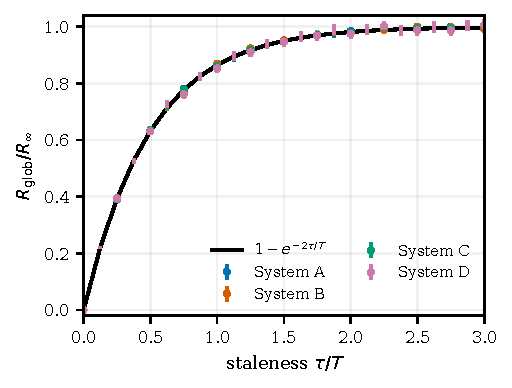
\includegraphics[width=0.82\linewidth]{figures/fig7_1_temporal_scaling.pdf}
\caption{Temporal scaling collapse. Markers are Monte Carlo estimates for four
systems with different dimensions, spatial covariances, objective matrices,
and decision operators; bars are 95\% confidence intervals. The solid curve
is the exact law $1-e^{-2\tau/T}$. Normalization by $R_\infty$ removes all
system-specific scale.}
\label{fig:temporal-scaling}
\end{figure}

We next used the shared-resource model
$Q=qI+\gamma\mathbf 1\mathbf 1^\top$, $q=1$, with independent OU components.
Figure~\ref{fig:local-global-phase} compares the empirical crossover with the
exact finite-$n$ threshold in Eq.~\eqref{eq:aggregate_rho_star}.  Over 36
$(n,\gamma/q)$ settings, the mean absolute boundary error was $0.00111$ and
the maximum was $0.00557$.  Finite size matters most under strong coupling:
at $n=5$ and $\gamma/q=10$, the exact threshold is $0.109$ below the
large-system limit.  As $n$ grows, the measured boundary approaches
$\tfrac12\log(1+\gamma/q)$, confirming that stronger decision coupling
increases the amount of global staleness worth tolerating.

\begin{figure}[t]
\centering
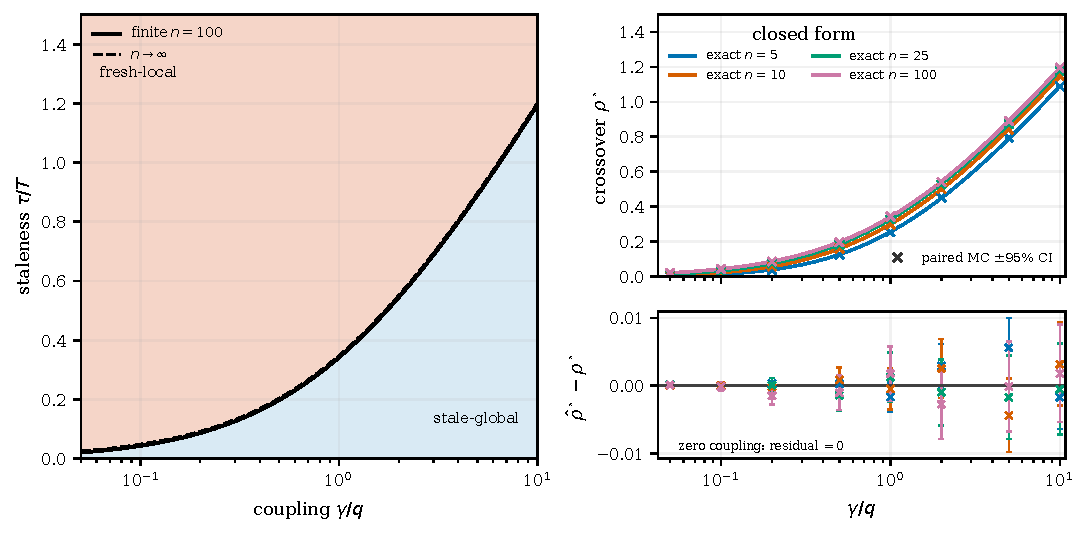
\includegraphics[width=0.98\linewidth]{figures/fig7_2_local_global_phase.pdf}
\caption{Fresh-local versus stale-global crossover. Left: winning architecture
for $n=100$; the solid finite-$n$ boundary and dashed large-$n$ boundary are
Eqs.~\eqref{eq:aggregate_rho_star} and \eqref{eq:large_n_threshold}.
Right: covariance boundaries (lines) and Monte Carlo estimates (crosses) for
four system sizes. Stronger coupling makes older global information worth
tolerating.}
\label{fig:local-global-phase}
\end{figure}

\subsection{Emergence of an Optimal Coordination Radius}
\label{subsec:numerical-radius-curves}

To expose the full tradeoff, we used
$\eta_S(r)=\eta_0e^{-2r/\ell_c}$, $\tau(r)=r/v$, and decomposed regret into
the terms $R_T(r)$ and $R_S(r)$ of Eq.~\eqref{eq:R_decomposition}.
Figure~\ref{fig:radius-regret} deliberately selects local, interior, and
boundary/global regimes on $0\le r/\ell_c\le2$.  The grid minimizers were
$0$, $0.626$, and $2.000$, respectively; the analytical capped optima were
$0$, $0.62638$, and $2.000$.  In the interior case the numerical radius error
was $3.81\times10^{-4}$ and
$|m_S(\hat r^\star)-m_T(\hat r^\star)|=4.77\times10^{-4}$, directly testing
Eq.~\eqref{eq:marginal_balance_condition}.  Independent innovation sampling
tracked the covariance curves with a worst-case absolute deviation of $0.020$
over all radii and all three regimes.

\begin{figure}[t]
\centering
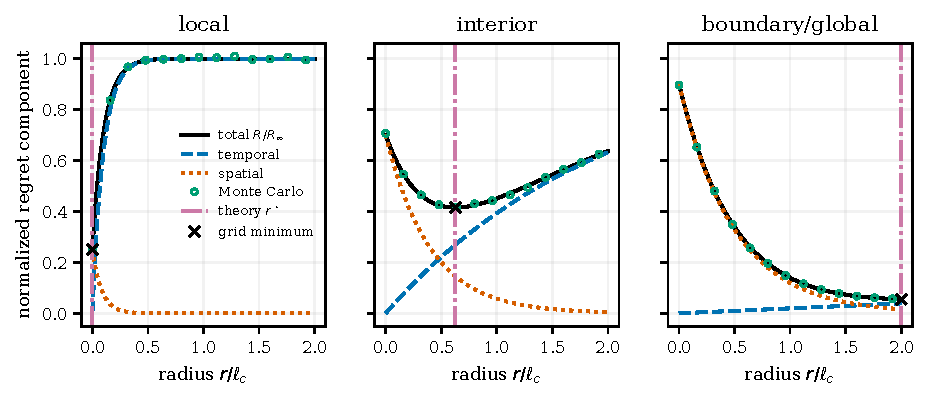
\includegraphics[width=\linewidth]{figures/fig7_3_radius_regret.pdf}
\caption{Emergence of local, interior, and boundary/global optima under
$\eta_S(r)=\eta_0e^{-2r/\ell_c}$ and $\tau(r)=r/v$. Curves show total regret
and its temporal and residual-spatial terms from Eq.~\eqref{eq:R_decomposition};
open circles are independent Monte Carlo estimates. Dash-dotted lines and
crosses mark the analytical and grid minimizers.}
\label{fig:radius-regret}
\end{figure}

\subsection{Scaling Laws and Regime Map}
\label{subsec:numerical-radius-phase}

We swept 4,896 points over
$vT/\ell_c\in[0.1,20]$ and $\ell_s/\ell_c\in[0.05,5]$.  At each point we
minimized Eq.~\eqref{eq:regret_composition_normalized} on a 2,501-point radius
grid independently of the closed form.  Figure~\ref{fig:radius-phase} shows
the predicted zero-to-positive-radius threshold at $vT=2\ell_s$ and the quantitative agreement with
Eq.~\eqref{eq:canonical_dimensionless_law}: mean absolute radius error
$2.25\times10^{-4}$, maximum error $8.00\times10^{-4}$, against a maximum
grid spacing $1.60\times10^{-3}$.  Five grid points immediately adjacent to
the transition were classified as zero rather than positive because their
closed-form optima fell below one grid step; there were no discrepancies away
from that resolution band.  Separate one-dimensional numerical sweeps were
monotone in all four predicted directions: $r^\star$ increased with $T$, $v$,
and $\ell_c$, and decreased with $\ell_s$.

\begin{figure}[t]
\centering
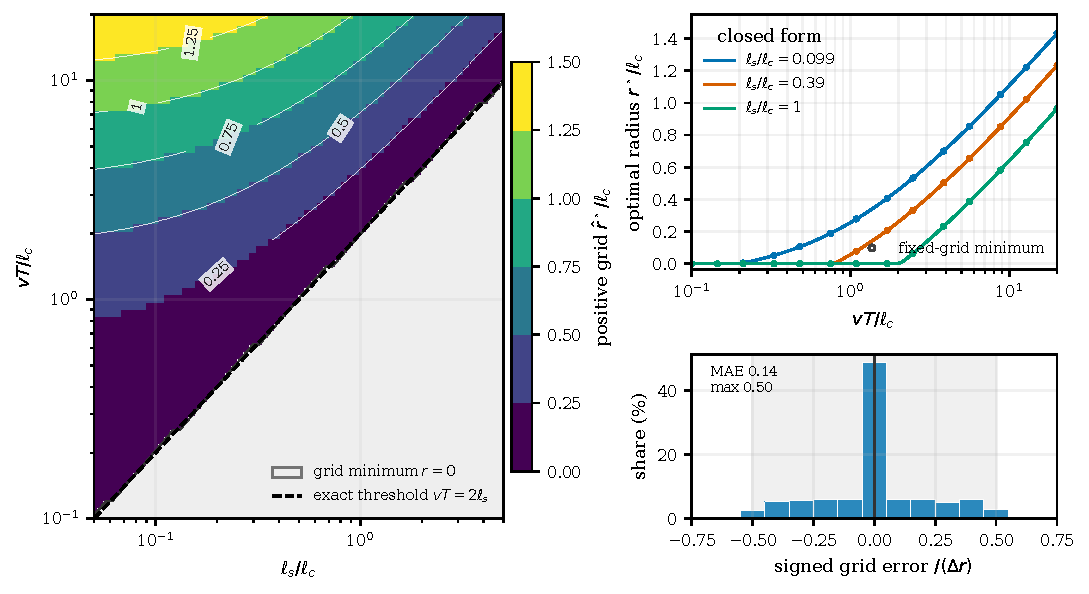
\includegraphics[width=0.98\linewidth]{figures/fig7_4_radius_phase.pdf}
\caption{Dimensionless optimal-radius law. Left: numerical
$r^\star/\ell_c$ over the $(\ell_s/\ell_c,vT/\ell_c)$ plane; the dashed line
is the predicted transition $vT=2\ell_s$. Right: grid minimizers versus the
closed form in Eq.~\eqref{eq:canonical_dimensionless_law}; the dashed line is
equality.}
\label{fig:radius-phase}
\end{figure}

\subsection{State Predictability versus Decision-Relevant Predictability}
\label{subsec:numerical-decision-relevance}

We next held a 64-node ring, its Laplacian covariance, $T=6$, and the latency
law fixed, changing only the normalized decision-sensitivity operator
$K_{ij}\propto e^{-d_G(i,j)/\ell_c}$.  Exact Gaussian conditioning gives the
curves in Fig.~\ref{fig:decision-relevance}.  Increasing $\ell_c$ from $0.7$
to $2$ to $6$ increased $\eta_S(0)$ from $0.0460$ to $0.258$ to $0.572$ and
moved the discrete optimum from 1 to 2 to 5 hops, even though the raw state
correlation was identical.  Monte Carlo conditioning checks differed from the
exact $\eta_S(r)$ by at most $3.12\times10^{-4}$.  Thus the same stochastic
environment supports substantially different architectures depending on
which spatial modes affect the desired decision.

\begin{figure}[t]
\centering
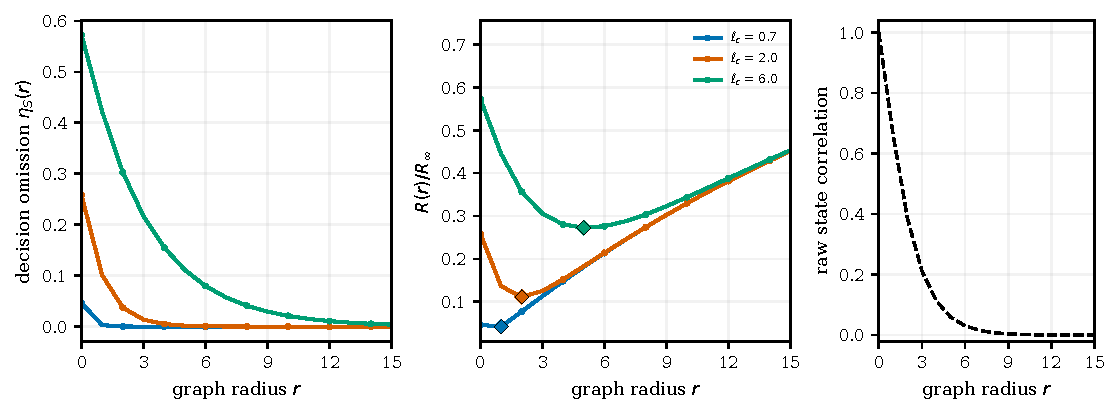
\includegraphics[width=0.94\linewidth]{figures/fig7_5_decision_relevance.pdf}
\caption{Decision relevance with the graph and state covariance held fixed.
Left: exact Gaussian spatial omission for three normalized decision operators;
the dashed raw state correlation is identical in every case. Right: composed
regret with the minimizing radius marked. Changing only the decision-relevance
range moves the optimum from 1 to 5 hops.}
\label{fig:decision-relevance}
\end{figure}

\subsection{Beyond the Canonical Line Model}
\label{subsec:numerical-general-graphs}

Finally, we considered 64-node path, ring, two-dimensional grid, and random
geometric graphs.  For each graph we formed
$\Sigma_S=(\kappa_s^2I+L_G)^{-\nu}$, normalized its marginal variance, and
computed every $\eta_S(r)$ directly from the Gaussian conditional covariance
of the desired action given the radius-$r$ neighborhood.  No exponential fit
or canonical line formula was used.  Under the common reference setting,
Fig.~\ref{fig:general-graphs} gives optima of 2, 2, 3, and 2 hops for the path,
ring, grid, and geometric graph, respectively.

Across all four graph classes, increasing $T$ from $1.5$ to $14$ changed the
optimal radius from 1 to 3 hops on the path and ring, from 1 to 4 on the grid,
and from 1 to 3 on the geometric graph.  Increasing the decision range from
$0.7$ to $6$ moved the corresponding endpoints from $(0,0,1,1)$ to
$(5,5,5,3)$.  Increasing per-hop latency weakly decreased every optimum.
Spatial smoothness was increased by decreasing $\kappa_s$ (which emphasizes
low graph frequencies after variance normalization); the optimal radii weakly
decreased, as broader measurements became more redundant.  Because radius is
discrete, these stepwise changes should be interpreted using one-hop regret
differences---the discrete analogue of marginal balance---rather than the
continuous first-order condition in Eq.~\eqref{eq:marginal_balance_condition}.

\begin{figure}[t]
\centering
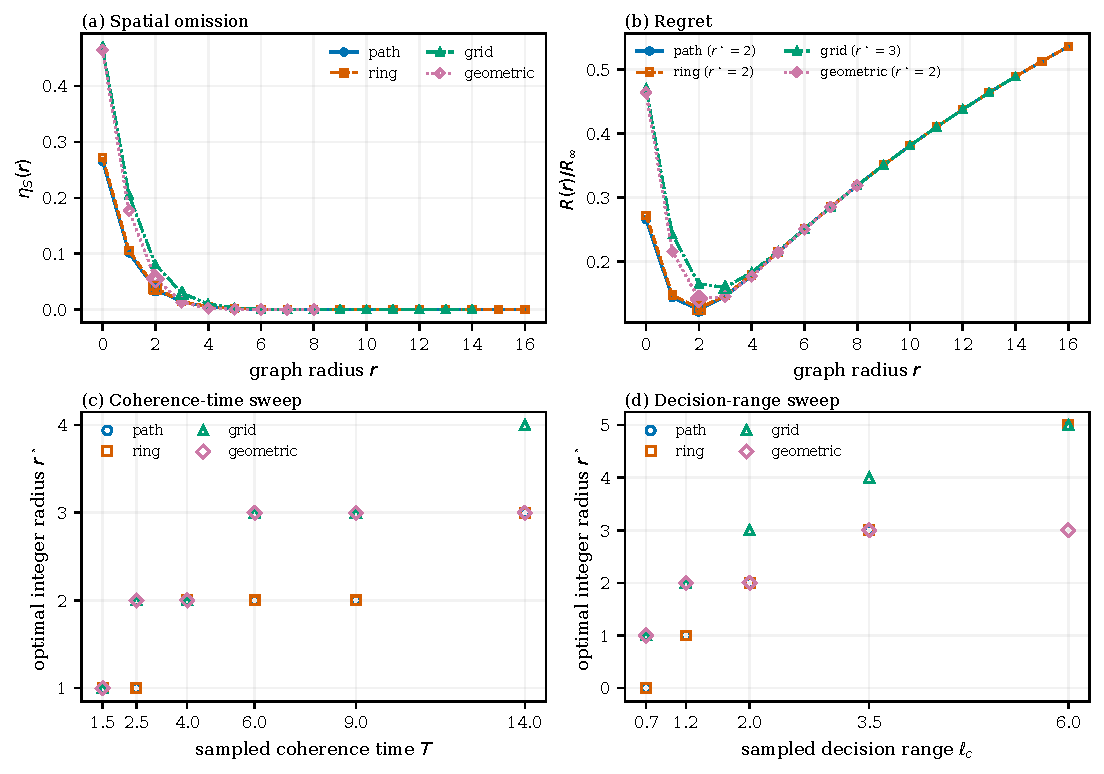
\includegraphics[width=0.94\linewidth]{figures/fig7_6_general_graphs.pdf}
\caption{Finite noncanonical graphs. Top: $\eta_S(r)$ computed from actual
Gaussian conditional covariances and the resulting regret under one common
normalized setting. Bottom: discrete optimal radius versus coherence time and
decision-relevance range. The canonical line closed form is not used; the
stepwise shifts are the discrete analogue of marginal balance.}
\label{fig:general-graphs}
\end{figure}
\clearpage

\section{Related Work}

\subsection{Static Team Decision Theory}

Radner established foundational optimality conditions for static teams, in which decision makers share a common objective but act on different information \cite{radner1962team}. Under appropriate convexity and regularity conditions, the resulting stationarity conditions are sufficient for global team optimality; in the quadratic Gaussian specialization, the optimal decision rules are affine \cite{radner1962team,marschak1972economic}. In the deterministic-Hessian quadratic model used here, these fixed-information optimality conditions admit the equivalent Hilbert-space formulation developed in Section~\ref{subsec:projection}: for a fixed information architecture $\mathcal A$, the team-optimal policy is the $Q$-orthogonal projection of the full-information action onto the closed subspace $\mathcal S(\mathcal A)$ of implementable policies. This projection identity is a specialization of the classical static-team framework to our quadratic model, rather than the literal statement of Radner's theorem. Krainak, Speyer, and Marcus subsequently relaxed the sufficient conditions associated with Radner's stationarity result and extended the theory to an exponential-quadratic criterion with jointly Gaussian state and observations \cite{krainak1982staticI}. In a companion paper, they formulated affine linear-quadratic-Gaussian and linear-exponential-Gaussian team problems as constrained parameter optimizations and represented optimal team gains as projections of the corresponding centralized gains \cite{krainak1982staticII}.

Classical team theory also treated information itself as an organizational design object. Marschak and Radner analyzed the value of information, delayed information and the tradeoff between timeliness and completeness, and formulated team organization in terms of optimal networks \cite{marschak1972economic}. More recently, Summers, Li, and Kamgarpour formulated information-structure design as the selection of additional measurements or communication links jointly with the corresponding team decision strategies \cite{summers2017information}. Afshari and Mahajan characterized quadratic Gaussian static teams whose observations decompose into information common to all agents and agent-specific local information \cite{afshari2017static}. They subsequently applied this decomposition to team-optimal decentralized filtering over communication graphs with delayed information sharing, where sufficiently old measurements constitute common information while more recent measurements remain local \cite{afshari2018team}. Rusmevichientong and Van Roy studied large teams in which each agent observes the local cost structure only within a graph radius, using centralized performance as a benchmark \cite{rusmevichientong2003decentralized}. Gamarnik, Goldberg, and Weber studied decentralized decisions based on local information in random decision networks and related their near-optimality to a correlation-decay, or long-range-independence, property \cite{gamarnik2014correlation}.

Relative to these works, the distinctive object studied here is a structured family of information architectures in which spatial scope and temporal freshness are coupled through the scope--latency relation $\tau(r)$. Delayed information and timeliness--completeness tradeoffs are already present in classical team theory \cite{marschak1972economic}, while prior information-structure-design work selects additional information links \cite{summers2017information} and prior local-information models study performance as a function of information radius \cite{rusmevichientong2003decentralized}. Here, instead, each spatial scope induces an acquisition delay, and the resulting architecture is valued through its prediction error for the full-information decision. This coupling yields the freshness--locality crossover and coordination-scale laws developed in Sections~\ref{sec:fresh_local_global} and \ref{sec:optimal_coordination_scale}.

\subsection{Distributed Optimization and Networked Control}

Distributed optimization studies how agents compute a common solution using local computation and message exchange. Classical asynchronous gradient methods allow delayed interprocessor communication while retaining convergence guarantees under suitable boundedness conditions \cite{tsitsiklis1986distributed}, while distributed subgradient methods establish convergence when agents exchange information locally over time-varying network topologies \cite{nedic2009distributed}. In these canonical formulations, the communication process constrains an iterative computation of an optimizer. Our setting separates that computational question from information architecture: the full-information decision at each epoch is the benchmark, and the object of design is the information available when that decision must be made.

Networked and decentralized control instead place communication constraints directly in the feedback loop, including sampling, delay, and packet loss \cite{hespanha2007survey}. Spatially distributed control has long imposed finite-speed information propagation, including communication delay proportional to spatial distance \cite{voulgaris2003optimal}, and subsequent work has co-designed communication architecture and closed-loop performance \cite{matni2017communication}. Most directly, Ballotta, Jovanovi\'c, and Schenato parameterize controller architectures by communication scope together with an increasing architecture-dependent latency, and show that sparse nearest-neighbor feedback can outperform all-to-all control \cite{ballotta2023latency}; subsequent work studies how communication delays reshape the locality of optimal feedback \cite{ballotta2026role}. Thus the distinction here is not the existence of a scope--delay tradeoff. These works study dynamic plants in which feedback affects future state evolution, whereas our environment evolves exogenously and each epoch is a static team decision. Spatial scope induces information age through $\tau(r)$, and architectures are valued by the resulting prediction error for the current full-information decision. This yields the freshness--locality crossover and optimal coordination-scale laws in terms of decision-relevant predictability rather than closed-loop dynamics.

\subsection{Freshness and Age of Information}

Age of Information (AoI) formalizes the timeliness of status information through the age of the freshest received update, $\Delta(t)=t-u(t)$. Seminal work showed that minimizing AoI is distinct from maximizing throughput or minimizing packet delay and initiated a large literature on update generation, queueing, and scheduling \cite{kaul2012realtime,yates2021aoi}. Subsequent work generalized linear age to application-specific nonlinear age penalties \cite{sun2017update}. Connections to remote estimation make the distinction between age and task loss explicit: for a Gauss--Markov Ornstein--Uhlenbeck process, estimation error under signal-agnostic sampling is a nonlinear function of age, whereas signal-aware sampling can exploit the realized estimation error and outperform age-optimal policies \cite{ornee2021ou}.

More recent work has pushed freshness metrics toward task-aware objectives. Shisher et al. showed that remote-inference loss can be nonmonotonic in age and designed communication policies around inference performance \cite{shisher2024timely}; subsequent work considers correlated sources for which inference penalties depend jointly on multiple sources' ages \cite{shisher2026correlated}. Li et al. go further toward decision-aware freshness by jointly optimizing sampling and remote decision making under stale observations \cite{li2026freshness}. Our problem is complementary but distinct. Rather than optimizing when or which updates to transmit to a fixed remote receiver, we choose the information architecture available to a decentralized team---what is observed, from what spatial scope, and at what age. Because broader scope itself incurs greater acquisition delay, spatial omission and temporal staleness are coupled by the architecture. This leads to the fresh-local/stale-global crossover and optimal coordination-scale results developed here.

\subsection{Centralization, Delegation, and Organizational Economics}

A closely related organizational-economics literature asks how dispersed information, communication constraints, and decision rights determine organizational form. Aoki compares hierarchical and horizontal information structures when local conditions are uncertain and central monitoring or response is limited \cite{aoki1986horizontal}. In the information-processing tradition, Radner studies organizations of limited-capacity processors trading off processing resources against decision delay \cite{radner1993organization}; Bolton and Dewatripont derive communication networks from processing and communication costs \cite{bolton1994firm}; and Van Zandt studies real-time decentralized processing in which computational delay constrains the use of recent information \cite{vanzandt1999realtime}. Dessein and Santos likewise study adaptation to local information versus coordination under imperfect communication \cite{dessein2006adaptive}.

A complementary delegation literature makes decision rights endogenous when information and objectives are dispersed. Aghion and Tirole distinguish formal from real authority \cite{aghion1997formal}, while Dessein studies delegation as an alternative to strategic communication \cite{dessein2002authority}. Most closely related to our centralization framing, Alonso, Dessein, and Matouschek compare centralized and decentralized coordination when managers privately observe local conditions \cite{alonso2008coordination}. Our model deliberately abstracts from incentive conflicts and endogenous information acquisition: agents share a common objective and the environment evolves exogenously. The tradeoff studied here is spatio-temporal: broader synchronized snapshots can improve coordination but arrive older. This yields a pure-benchmark crossover and, in the canonical spatial model, an interior optimum within the synchronized-snapshot family.

\subsection{Spatial Statistics and Graph Signal Processing}

Spatial statistics provides the closest statistical antecedent to our spatial-predictability model. Kriging casts spatial prediction as an optimal linear prediction problem under spatial dependence \cite{cressie1990origins}. For lattice data, Besag's conditional formulation represents spatial dependence through local Markov neighborhoods \cite{besag1974spatial}; Lindgren, Rue, and Lindstr\"om later connect Mat\'ern Gaussian fields to sparse Gaussian Markov random fields through stochastic partial differential equation representations \cite{lindgren2011explicit}. Space--time statistics likewise treats separability as a modeling restriction rather than a necessity: Gneiting constructs broad classes of stationary nonseparable covariance functions \cite{gneiting2002nonseparable}. These works provide the statistical context for our covariance-based spatial model and its separable/nonseparable distinction.

Graph signal processing extends analogous ideas to irregular domains. Shuman et al.\ use graph-Laplacian eigenvectors to define a graph Fourier domain and associate low graph frequencies with signals that vary slowly over the graph \cite{shuman2013emerging}. Graph-sampling theory asks when bandlimited graph signals can be exactly recovered from partial observations \cite{chen2015discrete}, while stationary graph signal processing gives spectral descriptions and Wiener-type estimators for random graph signals \cite{perraudin2017stationary}. Our objective is different: we do not value accurate reconstruction of $\theta_t$ per se. A radius-$r$ architecture is evaluated by its loss in reproducing the full-information decision $x_t^\star$, and increasing $r$ also increases information age through $\tau(r)$. Thus spatial omission and temporal staleness are priced jointly, and graph-smooth modes matter only insofar as they are decision-relevant.

\iffalse % Superseded implications/extensions and conclusion retained inactive.
\section{Architectural Implications and Extensions}
\label{sec:implications}

The preceding results suggest viewing information architecture itself as a
design variable. The local--global crossover identifies when freshness should
be preferred to breadth, while the optimal-radius result identifies the spatial
scale at which additional information ceases to justify the delay required to
obtain it. This section summarizes the resulting design implications, clarifies
the principal modeling limitations of the present theory, and outlines several
directions for extending it.

\subsection{From Local to Global Architectures}

The results of Sections~\ref{sec:fresh_local_global} and
\ref{sec:optimal_coordination_scale} imply that neither purely local nor fully
global information is universally preferable. Instead, the appropriate
architecture depends on the interaction among temporal coherence, spatial
predictability, communication latency, and decision coupling.

When the environment changes rapidly relative to information-propagation time,
or when remote state is highly predictable from local observations, a small
information radius is favored. Conversely, slow temporal variation, fast
information propagation, or strong long-range decision coupling make broader
information more valuable. Intermediate-radius architectures arise naturally
when the marginal benefit of additional spatial information balances the
freshness loss incurred in obtaining it.

This perspective replaces the usual binary distinction between centralized and
distributed decision making with a continuum of architectures,
\begin{equation}
    \mathcal{A}_{0}
    \longrightarrow
    \mathcal{A}_{r}
    \longrightarrow
    \mathcal{A}_{D},
    \label{eq:architecture_continuum}
\end{equation}
ranging from fresh-local to delayed-global information. The optimal operating
point on this continuum is determined by the decision problem and the
spatio-temporal statistics of the environment rather than by architecture
labels alone.

Information also need not be transported in raw form. If the globally optimal
decision depends on remote state only through a low-dimensional statistic,
then disseminating that statistic may provide most or all of the coordination
benefit at substantially lower latency. This motivates hybrid architectures of
the form
\begin{equation}
    \text{fresh local state}
    \quad+\quad
    \text{low-dimensional global summary},
    \label{eq:hybrid_architecture_principle}
\end{equation}
such as congestion prices, aggregate resource signals, or other
decision-relevant summaries.

\subsection{Designing the Information Topology}

The radius-dependent architectures analyzed in this paper impose a regular and
symmetric information structure. More general systems may benefit from
nonuniform information topologies. A node need not receive all state within a
fixed radius, nor must all nodes use the same radius.

Let $\mathcal{A}$ denote any admissible information architecture and let
$C(\mathcal{A})$ represent its communication, sensing, computation, or monetary
cost. A natural extension is
\begin{equation}
    \min_{\mathcal{A}}
    \;
    R(\mathcal{A})
    +
    \lambda C(\mathcal{A}),
    \label{eq:architecture_regularized_design}
\end{equation}
or equivalently
\begin{equation}
    \min_{\mathcal{A}}
    \;
    R(\mathcal{A})
    \qquad
    \text{s.t.}
    \qquad
    C(\mathcal{A})\le B.
    \label{eq:architecture_budget_design}
\end{equation}

This is a significant extension of the present formulation. In the current
model, architecture regret measures only decision quality. Communication,
sensing, and computation costs enter indirectly through the set of feasible
architectures and, in particular, through the latency function $\tau(r)$.
In many practical systems these costs are themselves first-order design
considerations and should appear explicitly in the objective or as hard
resource constraints.

Such a formulation includes several practically relevant problems: selecting
which remote observations each agent receives, determining which information
links are worth maintaining, allocating update rates among different state
variables, and choosing how much bandwidth or computation to devote to
information acquisition.

If adding an observation or information link changes architecture
$\mathcal{A}$ to a richer architecture $\mathcal{A}'$, its decision value is
naturally measured by
\begin{equation}
    \Delta R
    =
    R(\mathcal{A})
    -
    R(\mathcal{A}').
    \label{eq:marginal_information_value}
\end{equation}
Thus information should be acquired not simply because it is uncertain, but
because resolving that uncertainty materially changes the downstream decision.

This viewpoint also suggests sparse, small-world-like information
architectures. A system may rely primarily on fresh local or neighborhood
state while maintaining only a small number of strategically selected
long-range information links. Such links can reveal spatial modes or remote
conditions that are poorly predicted locally but highly relevant to the
decision objective. Under suitable spatial structure, a sparse set of nonlocal
observations may therefore approach the decision quality of global information
without incurring the latency required to assemble a complete system-wide
snapshot.

The relevant information topology need not coincide with the physical
communication graph. The value of a long-range observation should depend on a
combination of
\begin{equation}
    \text{decision relevance}
    \times
    \text{statistical novelty}
    \times
    \text{freshness}
    \times
    \text{acquisition cost},
    \label{eq:information_link_value_factors}
\end{equation}
rather than physical distance alone.

\subsection{Adaptive and Sequential Information Acquisition}

The analysis so far assumes that the statistics governing spatial and temporal
predictability are known and stationary. In many systems these quantities must
instead be learned online and may themselves vary over time. Let
\begin{equation}
    \psi_t
    =
    \left(
        T_t,\ell_{s,t},\Sigma_t,\ldots
    \right)
    \label{eq:time_varying_statistics}
\end{equation}
denote time-varying parameters describing the current spatio-temporal
environment. An adaptive system could estimate $\psi_t$ from recent
observations and choose an architecture according to
\begin{equation}
    \mathcal{A}_t
    \in
    \arg\min_{\mathcal{A}}
    \left[
        \widehat{R}_t(\mathcal{A})
        +
        \lambda C(\mathcal{A})
    \right].
    \label{eq:adaptive_architecture_selection}
\end{equation}

This creates a natural separation of timescales: fast decisions are made using
the currently selected information architecture, while the architecture itself
is adapted more slowly as environmental statistics change. Such a formulation
could accommodate nonstationary regimes in which the preferred information
radius expands or contracts as spatial correlation, temporal coherence, or
decision coupling changes.

A related extension makes information acquisition sequential within a single
decision epoch. An agent may either act immediately using its current
information or wait for additional observations to arrive. Let
\[
    \mathcal{G}_{i}^{(0)}
    \subseteq
    \mathcal{G}_{i}^{(1)}
    \subseteq
    \cdots
\]
denote progressively richer information sets available after additional
waiting. The agent may choose a stopping time $\tau_i$ and then act using the
information available at that time. A stylized objective is
\begin{equation}
    \min_{\tau_i,u_i}
    \;
    \mathbb{E}
    \left[
        f(u_i,\theta)
        +
        C_{\mathrm{wait}}(\tau_i)
    \right].
    \label{eq:act_or_wait}
\end{equation}
The projection framework supplies the decision-regret term associated with
each information set, while optimal-stopping or sequential-decision methods
determine whether the expected reduction in regret justifies waiting.

More generally, an agent may choose not only whether to wait but
\emph{which} observation to request. This leads to adaptive information
acquisition policies in which remote measurements are queried only when their
expected decision value exceeds their communication, energy, or latency cost.

\subsection{Beyond the Canonical Statistical Model}

The closed-form results in this paper rely on deliberately strong modeling
assumptions. The exact projection geometry uses quadratic costs; the explicit
staleness and coordination-radius formulas additionally assume affine
full-information decisions, a common temporal coherence time for all modes,
and, for the canonical spatial result, a separable space--time covariance
model. These assumptions are analytically convenient and capture a useful
baseline class, but they exclude many practical networked decision problems.

For example, wireless power control and network utility maximization often
involve logarithmic or otherwise non-quadratic utilities; scheduling and
placement problems may involve discrete or combinatorial actions; and channel,
demand, or workload processes may be non-Gaussian, heavy-tailed,
mode-switching, or exhibit multiple temporal timescales. In such cases, the
specific formulas derived here should be interpreted as canonical design laws
rather than universal identities.

Several generalizations appear natural. For smooth strongly convex objectives,
quadratic approximation around the full-information optimum suggests that
architecture regret should remain locally controlled by a weighted
decision-prediction error, although exact projection identities become
upper--lower bounds. Multiple temporal timescales can be handled by replacing a
single coherence time $T$ with mode-dependent decay rates or, more generally,
a temporal prediction-error function. Likewise, nonseparable space--time
models can be treated through a joint predictability function
\begin{equation}
    \eta_{ST}(r,\tau),
    \label{eq:general_joint_predictability}
\end{equation}
without requiring the exact factorization obtained in
Theorem~\ref{thm:spatiotemporal_composition}. A broader theory should seek
architecture laws directly in terms of such decision-relevant predictability
functions rather than a particular Gaussian covariance family.

Combinatorial decision spaces present a more substantial departure, since the
set of feasible policies is no longer a linear subspace and the Hilbert-space
projection argument does not apply directly. Developing analogous notions of
architecture regret for discrete or constrained decisions is an important
direction if the framework is to cover scheduling, routing, placement, and
other common distributed-systems problems.

\subsection{Beyond Static Information Structures}

A second, more fundamental limitation is the restriction to static teams. The
environment may be highly correlated across space and time, but current actions
do not alter the law of future environmental states or the information later
observed by other agents. This exclusion is consequential because many
important networked systems operate precisely in the nonclassical regime.

Queue lengths depend on past routing and service decisions, battery states
depend on past energy expenditure, thermal states depend on previous
computation, and mobility decisions affect future channel and sensing
conditions. In these systems, the action is not merely a response to
information; it also changes the future state on which subsequent decisions
depend.

A modest first extension is to allow weak local action--state coupling,
\begin{equation}
    \theta_{i,t+1}
    =
    g_i(\theta_{i,t},w_{i,t})
    +
    \epsilon
    h_i(\theta_{i,t},x_{i,t},w_{i,t}),
    \label{eq:weak_dynamic_coupling}
\end{equation}
where $\epsilon$ quantifies the strength of the feedback. At $\epsilon=0$ the
present theory is exact. For small $\epsilon$, one may ask whether the
architecture rankings and coordination-scale laws obtained here remain stable
under perturbation. Such robustness results would extend the theory toward
systems with locally controlled queues, batteries, or resource states without
immediately confronting the full complexity of a general decentralized
dynamic program.

A sharper boundary is reached when one agent's actions influence what other
agents later observe. Then actions can serve both as controls and as implicit
signals, leading to the nonclassical dynamic-team phenomena highlighted by
Witsenhausen's counterexample
\cite{witsenhausen1968counterexample}. The static Hilbert-space projection
characterization no longer directly solves the problem.

Real backpressure routing illustrates this distinction. Queue lengths are
functions of past arrivals and service decisions and therefore are not
exogenous state variables in the sense assumed here. The present theory is most
directly interpreted in the rate or fluid domain, where demand, capacity,
channel state, or workload evolves externally and current decisions respond to
those quantities. Queue-based algorithms may realize related information
structures in practice, but their endogenous dynamics require additional
analysis.

Taken together, these extensions point toward a broader research question:
\begin{quote}
\emph{Given a distributed decision objective and an evolving environment, what
information should each agent acquire, from where, at what freshness, in what
representation, and at what cost before acting?}
\end{quote}
The present paper addresses a deliberately tractable first version of this
question by characterizing how spatial scope and temporal freshness determine
decision regret. Extending the framework to explicit information costs,
nonstationary statistics, sparse and adaptive information topologies,
sequential acquisition, non-quadratic and combinatorial decisions, and
controlled state evolution provides a natural path toward a more general
theory of information architecture for networked decisions.


\section{Conclusion}
\label{sec:conclusion}

This paper has studied a basic design question for networked decision systems:
how broad should the information available to each decision maker be when
obtaining information from farther away also makes that information less
fresh? We have formulated this question through information architectures that
specify the spatial scope and temporal age of the state available to each
agent.

Using the classical static-team projection characterization as an analytical
starting point, we have obtained two main results. First, we have derived an
exact fresh-local versus stale-global crossover law: local information becomes
preferable when the loss of temporal predictability in the delayed global
state exceeds the decision-relevant information unavailable locally. Under a
Gauss--Markov model, this has yielded a closed-form threshold in the ratio of
information delay to environmental coherence time. Second, we have generalized
the binary local--global comparison to radius-dependent information
architectures and have characterized the optimal coordination radius by
balancing marginal spatial information gain against marginal freshness loss.
In a canonical spatio-temporal model, this has produced an explicit scaling law
in terms of spatial correlation, temporal coherence, information-propagation
speed, and the spatial range of decision relevance.

The resulting picture is that the appropriate information architecture is
neither intrinsically local nor global. It is determined jointly by how
quickly the environment changes, how predictable remote state is from nearby
observations, how strongly remote state influences the desired decision, and
how quickly information can propagate through the network. Together, these
quantities determine a natural spatial scale of coordination.

The present theory has intentionally considered a tractable static-team setting
with quadratic costs and structured spatio-temporal statistics. Extending the
framework to explicit information-acquisition costs, adaptive and
nonstationary architectures, sparse long-range information links, sequential
act-or-wait decisions, non-quadratic or combinatorial objectives, and
action-dependent state evolution offers a broader path toward a theory of
information architecture for networked decisions.
\fi

\section{Discussion and Conclusions}
\label{sec:discussion_conclusions}

\paragraph{What the theory establishes.}
The central constraint in networked decision making is that information breadth
and freshness generally cannot be chosen independently. Nearby observations can
be used quickly but may omit remote state needed for coordination; a broader
view can improve coordination but loses predictive value while it is collected
and disseminated. An information architecture records this tradeoff by
specifying what each agent knows, from where, and at what age. Architecture
regret then measures the decision-quality loss relative to the full-information
decision after optimizing over every policy implementable under that
architecture. This separates the value of an information pattern from the
particular protocol or algorithm used to exploit it.

The fresh-local versus stale-global result characterizes the two endpoints.
Fresh-local information is preferred once the temporal unpredictability of the
delayed global history exceeds the fraction of decision-relevant variation
unavailable locally. Under the common-rate Gauss--Markov specialization, this
comparison depends on the dimensionless delay $\tau/T$ and the locally
captured share $\eta_{\mathrm{loc}}$. The closed form is useful because it
separates two mechanisms: the rate at which coordinated information ages and
the amount of the full-information decision already inferable from local
observations. The shared-resource example makes the second mechanism explicit:
stronger coupling raises the value of global coordination and therefore the
delay worth tolerating.

Intermediate radii define an outer design problem within the
synchronized-snapshot family. Increasing radius replaces a narrower, fresher
snapshot with a broader, older one. The optimum within this non-nested family
occurs where the proportional marginal gain in decision-relevant spatial
information equals the marginal loss of freshness.
In the canonical line model, the spatial correlation length $\ell_s$, the
decision-relevance length $\ell_c$, and the temporal propagation length
$L_T=vT$ determine the dimensionless radius and the transition
$L_T>2\ell_s$. The numerical experiments verify the temporal collapse and
local--global crossover, the zero-to-positive-radius threshold, the
predicted movement of the optimum, and the same marginal-balance behavior on
finite noncanonical graphs. Figures 1--4 provide implementation and
finite-sample verification, while Figs. 5--6 illustrate decision relevance and
finite-graph behavior. All experiments remain within the common-rate
Gaussian-affine model.

Normalizing by open-loop regret supports comparisons across the modeled
systems. It separates the overall scale of the decision problem from the
fraction of decision-relevant variation preserved by an architecture. Systems
with different dimensions, covariances, and coupling matrices can therefore
obey the same temporal law when they share the relevant normalized
predictability. The canonical formulas are exact, interpretable instances of
this comparison; the marginal-balance condition is the more general result
when spatial omission must instead be computed or estimated from the actual
graph.

\paragraph{Why decision-relevant predictability matters.}
Raw state predictability is not the correct design criterion. Architecture
regret depends on predicting the full-information decision $x^\star$, not on
reconstructing every component of $\theta$. A remote state component can be
hard to predict but architecturally unimportant when it has little influence on
the desired action. Conversely, a small residual uncertainty can matter when
the decision-sensitivity operator $K$ strongly amplifies that mode. The
relevant predictability therefore combines environmental statistics, decision
sensitivity and coupling, information geometry, and freshness. Holding the
state covariance fixed while varying $K$ in the numerical section demonstrates
that identical raw predictability can support substantially different optimal
coordination radii.

This distinction also separates physical communication geometry from decision
geometry. Graph distance determines which observations can be acquired and
their age on arrival; $Q$, $B$, and $K$ determine whether those observations
change the desired joint action. Two nearby nodes may be weakly coupled, while
distant nodes may interact strongly through a shared constraint or common
decision mode. An architecture based only on physical distance can therefore
communicate extensively about irrelevant variation while omitting a remote
mode with high decision value. Architecture design must use the communication
graph and the decision structure together.

The framework suggests broader information-architecture questions involving
topology, representation, and timing. The present results analyze scope and
timing for a synchronized-snapshot family; nonuniform topology and compressed
representation remain extensions.

\paragraph{Scope and deliberate limitations.}
The paper establishes an exogenous-state, static-team baseline. Environmental
state may be correlated across space and time, but current actions neither
alter its future law nor change what another agent later observes. Within this
boundary, the fixed-architecture quadratic projection gives an exact benchmark
for each fixed information pattern, and the paper's new results compare a
structured scope--age family using that benchmark. The principal radius family
uses synchronized snapshots. Under the common-rate Gaussian model,
Lemma~\ref{lem:snapshot_history_sufficiency} makes current snapshots sufficient
relative to observed histories for the affine current-decision prediction
problem; the equivalence is not assumed more generally.

The exact projection formula uses quadratic costs. The explicit stale-global
and composition laws additionally use affine full-information decisions and a
common-rate Gaussian or Gauss--Markov process, while the canonical radius
formula uses a separable homogeneous field and linear propagation delay. These
assumptions produce interpretable identities and dimensionless scaling laws.
The general lessons are broader than the canonical formula, but outside these
assumptions one should work directly with decision-relevant prediction-error
functions or suitable bounds rather than assume the same factorization. In
particular, nonquadratic and discrete decisions require analytical tools beyond
the Hilbert-space projection argument.

The exact projection characterization also assumes unconstrained Euclidean
action spaces. Nonnegativity, box, simplex, capacity, or other coupled
feasibility constraints generally replace the linear policy subspace by a
convex or nonconvex feasible set and require a different analysis. The
projection identities also assume a deterministic action Hessian $Q$; a
state-dependent or random Hessian may require a random weighted geometry and,
even under common information, need not reduce to the same ordinary
conditional-expectation formula.

The temporally evolving environment is treated as a sequence of stagewise
static teams: current actions neither alter later state, reshape another
agent's information, nor constrain later actions. The fixed-epoch projection
does not require stationarity; stationarity makes expected performance
time-invariant, while ergodicity is additionally needed for sample-path
long-run averages.

Finally, the common-rate assumption suppresses possible alignment between
temporal coherence, spatial scale, and decision relevance. If long-range
decision-relevant modes evolve more slowly than local modes, a scalar
common-rate approximation may understate the value of broad delayed
information; the reverse alignment may overstate it. There is no universal
direction of bias without specifying the mode weights and the procedure used
to select an effective coherence time. With heterogeneous temporal modes, the
scalar composition law generally gives way to a joint spatio-temporal
decision-prediction error.

\paragraph{Most important extensions.}
A first extension is to price information acquisition explicitly. The present
model represents communication and sensing constraints mainly through the
feasible scope--delay relationship. A richer problem would minimize
$R(\mathcal A)+\lambda C(\mathcal A)$, or impose a budget on
$C(\mathcal A)$, where cost may represent bandwidth, energy, sensing effort, or
computation. Explicit cost naturally leads to sparse and nonuniform topologies:
different agents need not use the same radius, and a small number of selected
long-range links may capture decision-relevant modes more efficiently than a
complete global view. When remote state matters mainly through a
low-dimensional statistic, compressed summaries may likewise retain most of
the coordination value while reducing latency.

A second extension is adaptation to unknown or nonstationary statistics.
Temporal coherence, spatial predictability, and decision sensitivity may need
to be estimated online, with the architecture changing on a slower timescale
than the operational decisions. The central challenge is then to account for
uncertainty in the estimated prediction-error functions while retaining a
stable architecture-selection rule.

An important extension is action-dependent state evolution and dynamic teams.
Queues depend on service and routing decisions, batteries on energy use,
thermal states on computation, mobility on previous control, and controlled
resources on earlier allocations. In such systems, actions alter future state
and may also signal information to other agents. The present static-team theory
deliberately establishes the exogenous-state baseline, while extending
information-architecture design to settings in which actions alter future state
and/or future information is an important next research direction.
Witsenhausen's counterexample \cite{witsenhausen1968counterexample} explains
why this is not a routine modification:
once control and signaling interact, the fixed-subspace projection
characterization generally no longer solves the team problem.

The present theory suggests the following design heuristic: expand information
scope only while the marginal decision value of broader information exceeds
the predictive value lost while obtaining it.

\paragraph{Code and data availability.}
The complete manuscript source, numerical code, configurations, raw and
processed results, and figure-generation pipeline are available in the TINA
reproduction repository \cite{tina2026software}. The cited release records the
exact submission version and immutable commit.

\bibliographystyle{IEEEtran}
\bibliography{references}


\end{document}
